\documentclass{article}
\usepackage[utf8]{inputenc}
\usepackage[left=1in,right=1in,top=1in,bottom=1in]{geometry}%


% AMS packages
\usepackage{amsmath}
\usepackage{amssymb}
\usepackage{amsthm}
\usepackage{mathtools}

% other packages
\usepackage{graphicx}
\usepackage{enumerate}
\usepackage{bbm}
\usepackage{float}

\graphicspath{ {images/} }

\usepackage{packages}

\title{Thouless pump}
\author{Ross Parker}

\begin{document}

\maketitle

\section{Introduction}

This is based on the Aubry-Andr\'e-Harper model of a quantized nonlinear Thouless pump in an array of coupled waveguides found in \cite{Jurgensen2021}. It is unclear which mathematical formulation we should use for the periodic waveguide coupling (options include mimicking Figure 1b and equation (3) in the supplement). Equation (3) in the supplement has the advantage that we get interesting solutions (both stationary and moving), some of which are stable. However, the coupling parameter in that equation can take negative values, which is nonphysical. Instead, we use the following equation, which essentially involves squaring equation (3) and the adjusting the parameters so that the period is what we want.
\[
J_n(z)= J_0 + C \cos^2\left(  \frac{2 pi}{3} n + \frac{\omega}{2} z + \frac{\pi}{6} \right).
\]
where $n$ is the index of the waveguide in the lattice \cref{fig:J}. Period is $T=2\pi$. The lattice dynamical system is then given by
\[
i \frac{d u_n}{d z} =
-J_n(z) u_{n+1} - J_{n-1}(z)u_{n-1} - g|u_n|^2 u_n,
\]
where we will (unless noted otherwise) take $g = 1$.

\begin{figure}
    \centering
    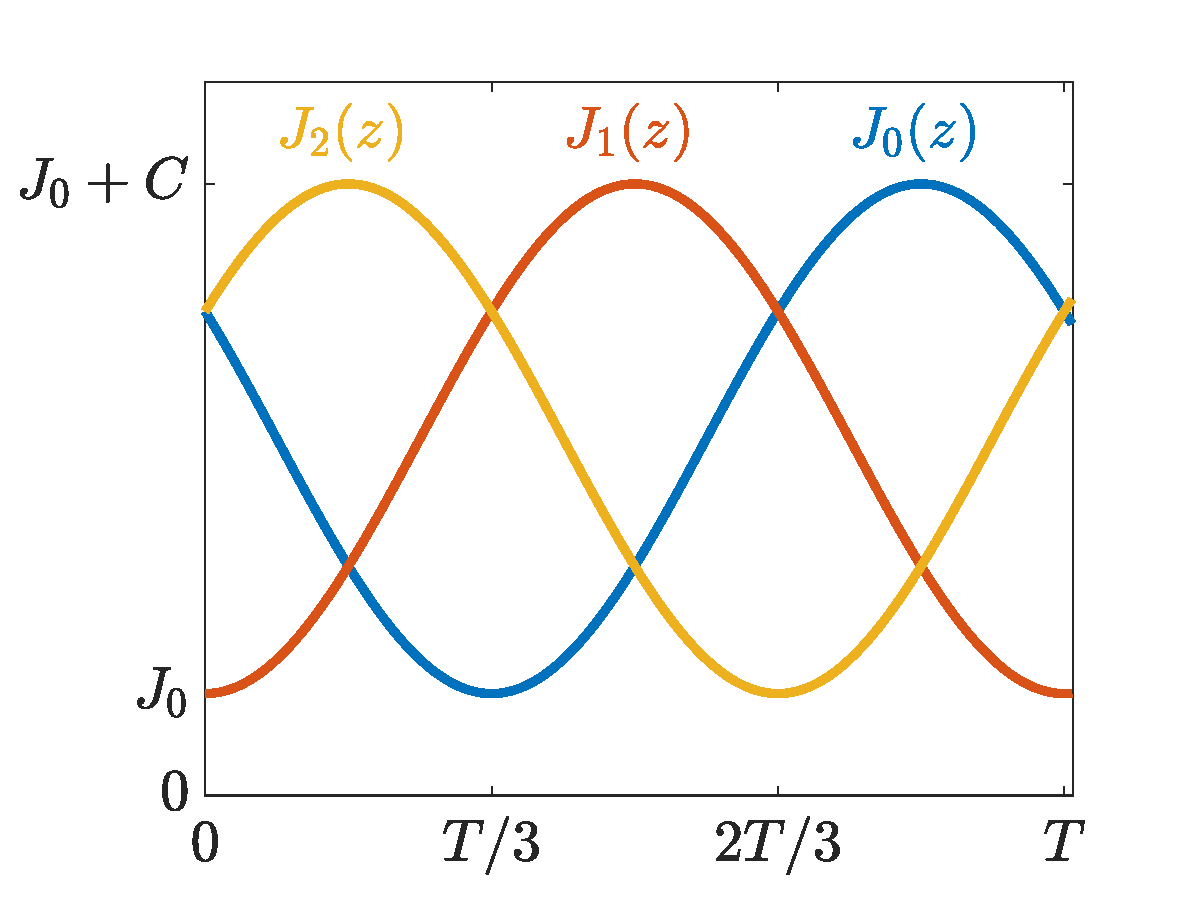
\includegraphics[width=7cm]{J}
    \caption{Coupling function $J_n(z)$ for $n = 0,1,2$.}
    \label{fig:J}
\end{figure}

\section{Evolution from single-site initial conditions}

\begin{figure}[H]
    \centering
    \begin{tabular}{cccc}
    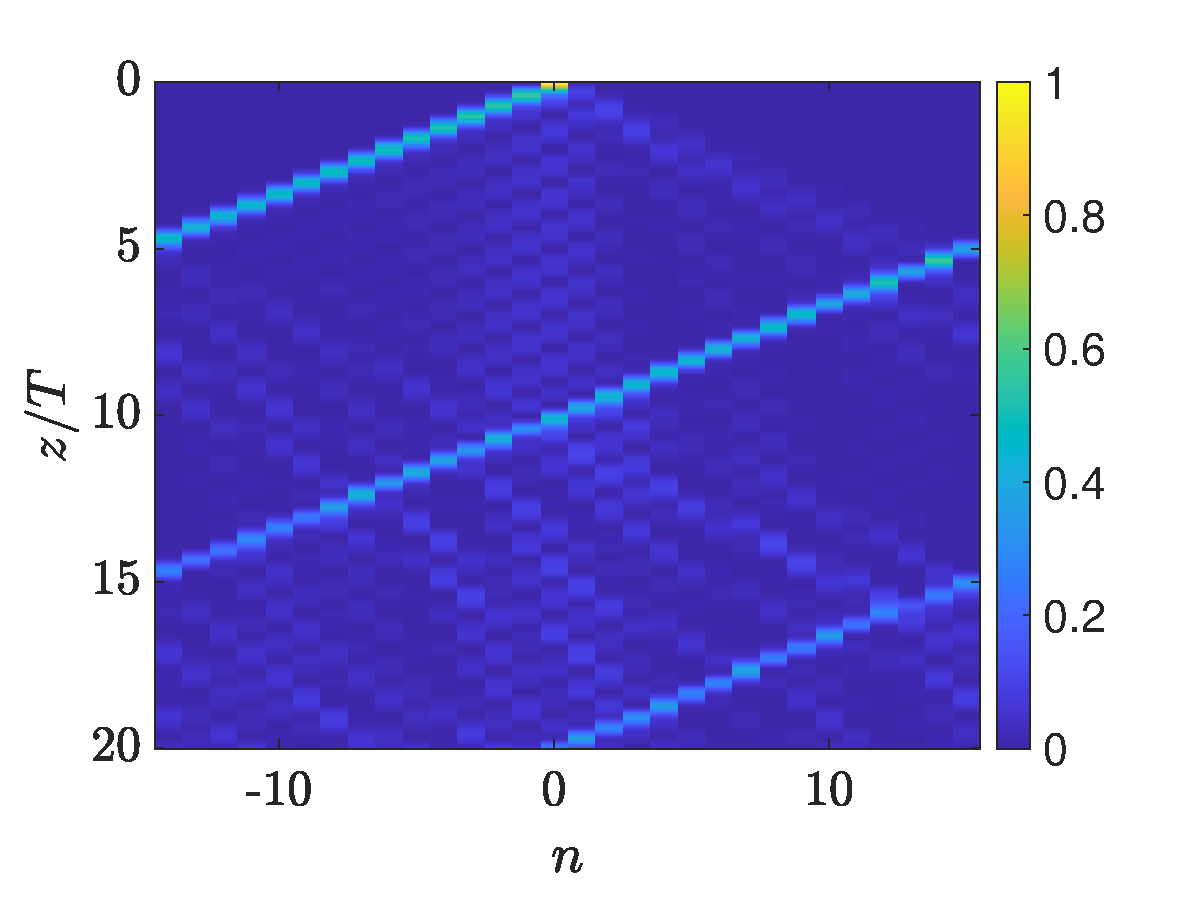
\includegraphics[width=4cm]{left1} &
    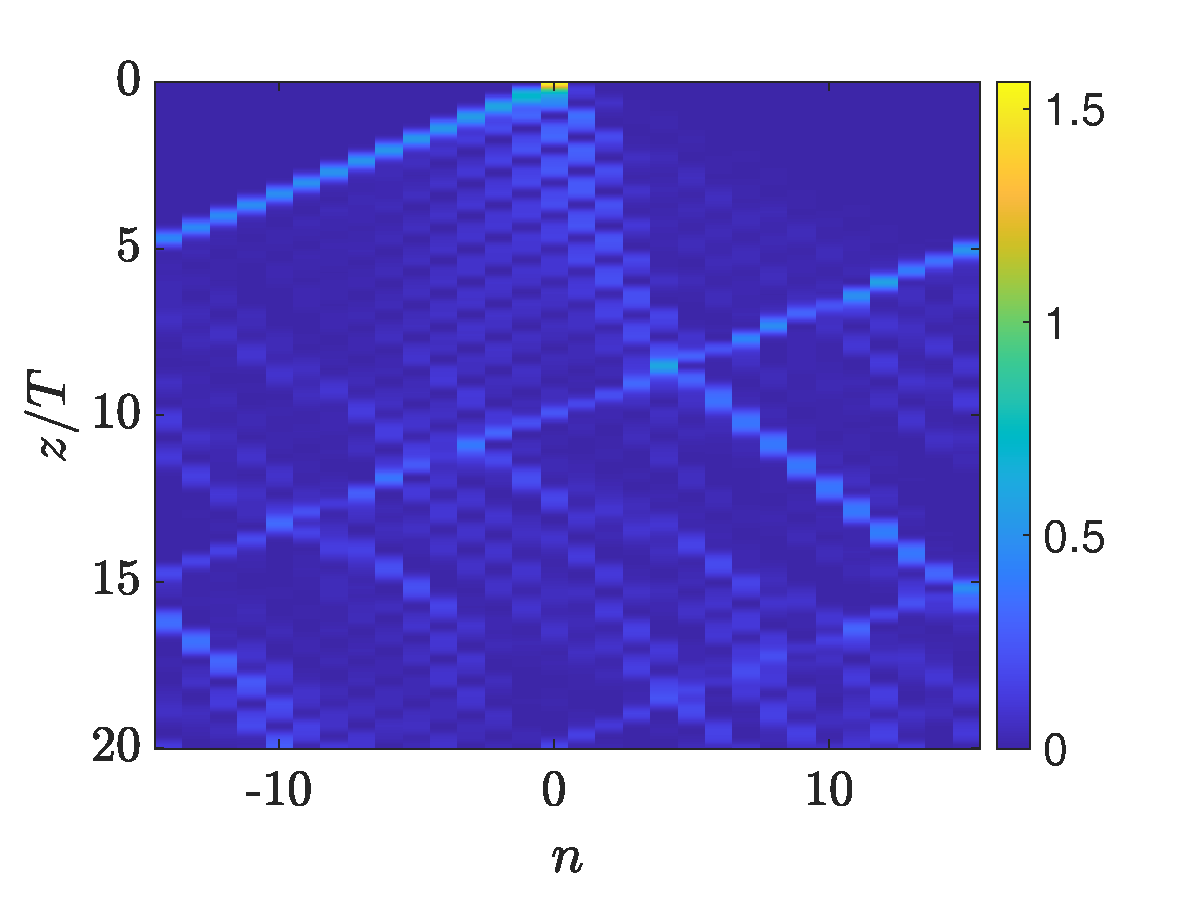
\includegraphics[width=4cm]{left125} &
    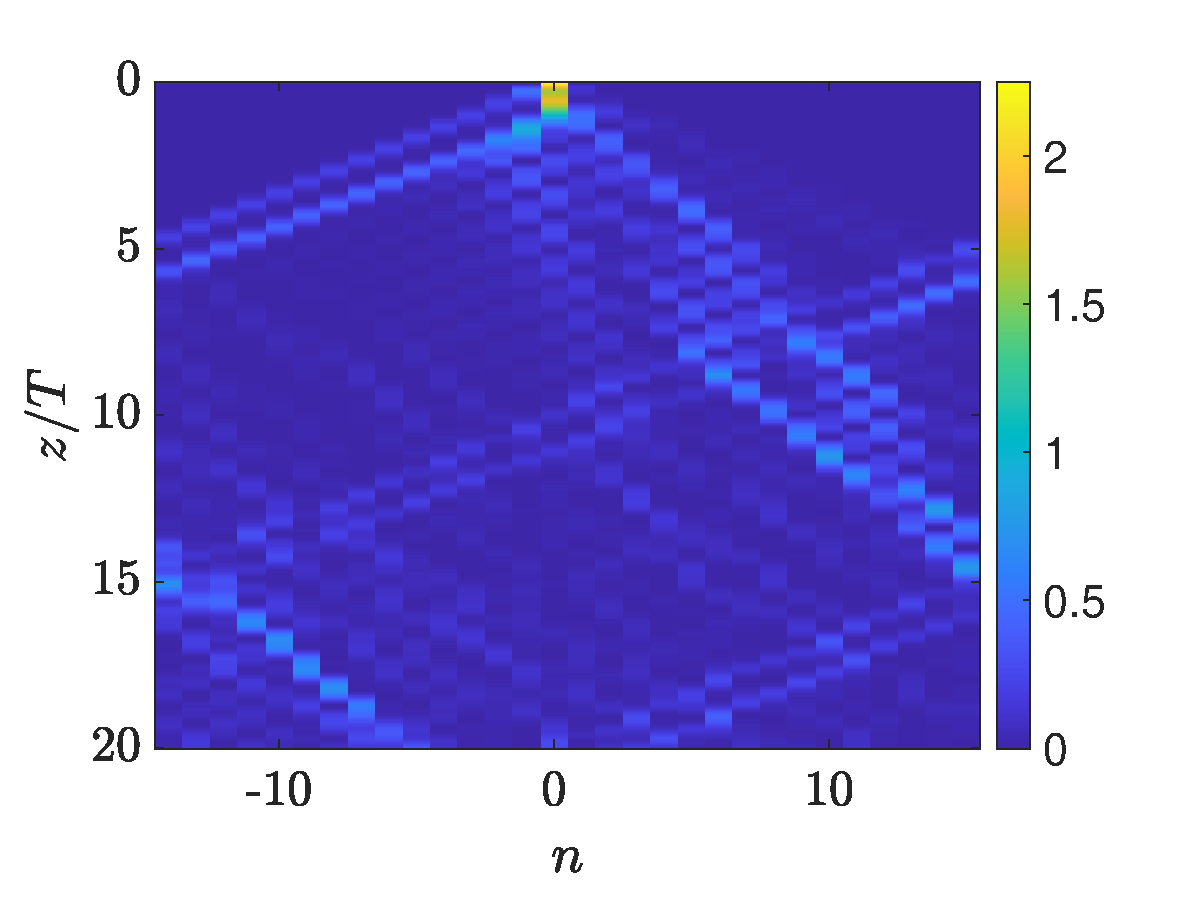
\includegraphics[width=4cm]{left15} &
    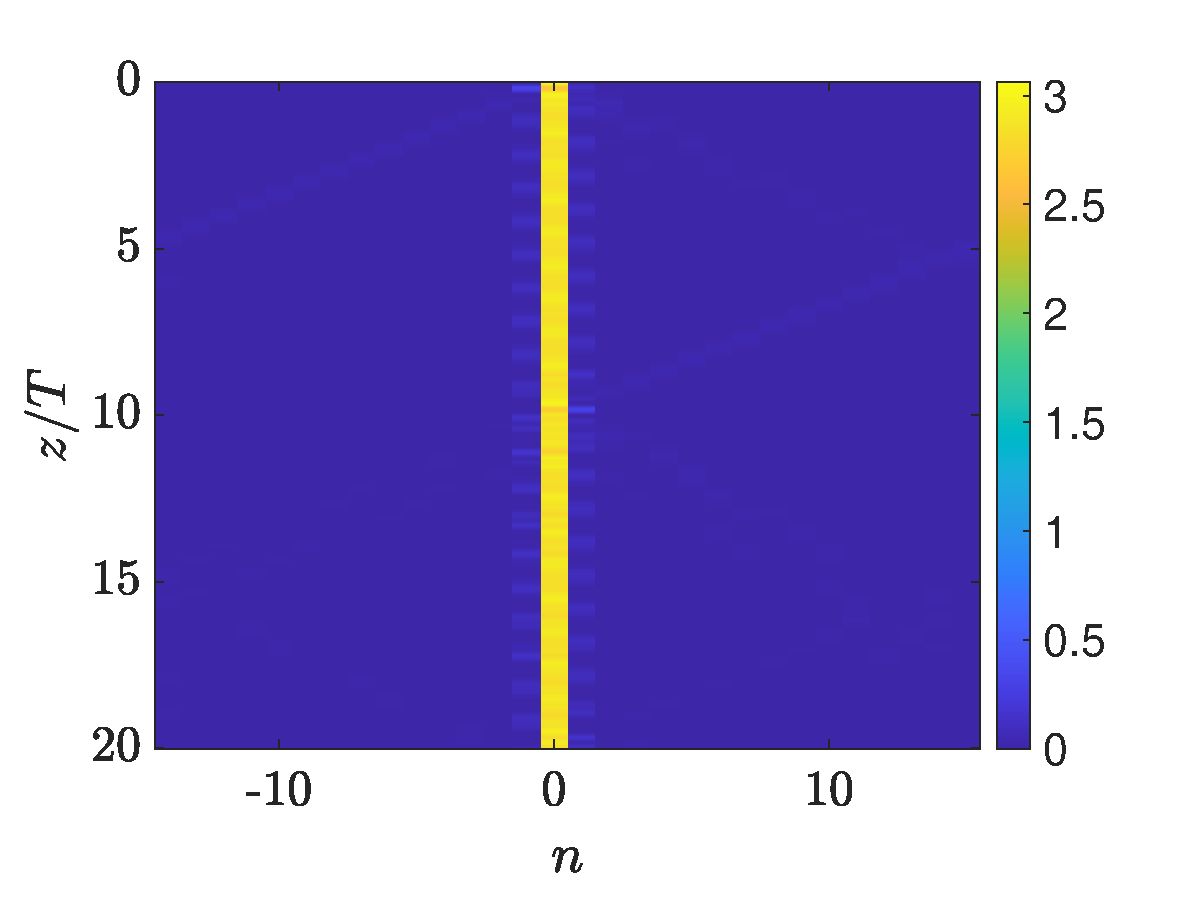
\includegraphics[width=4cm]{left175} \\
    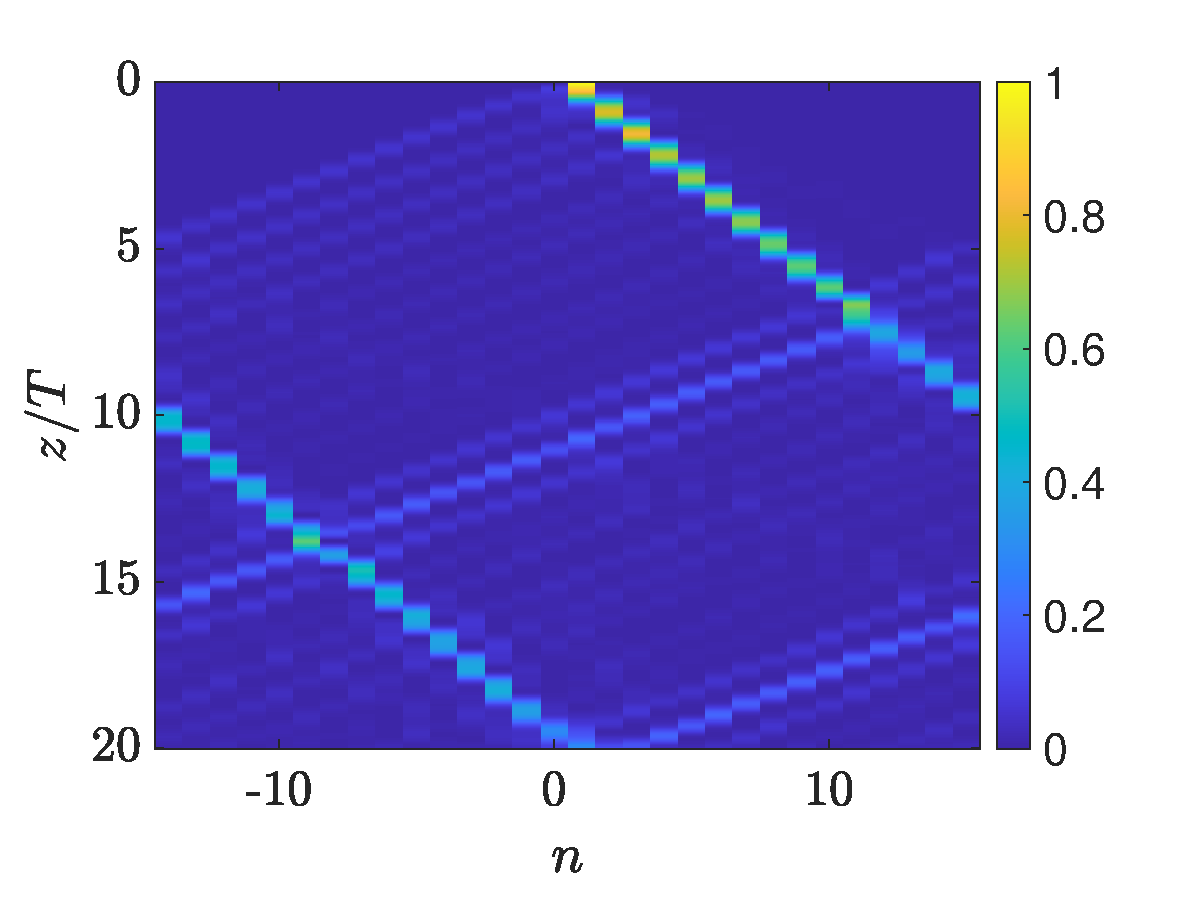
\includegraphics[width=4cm]{right1} &
    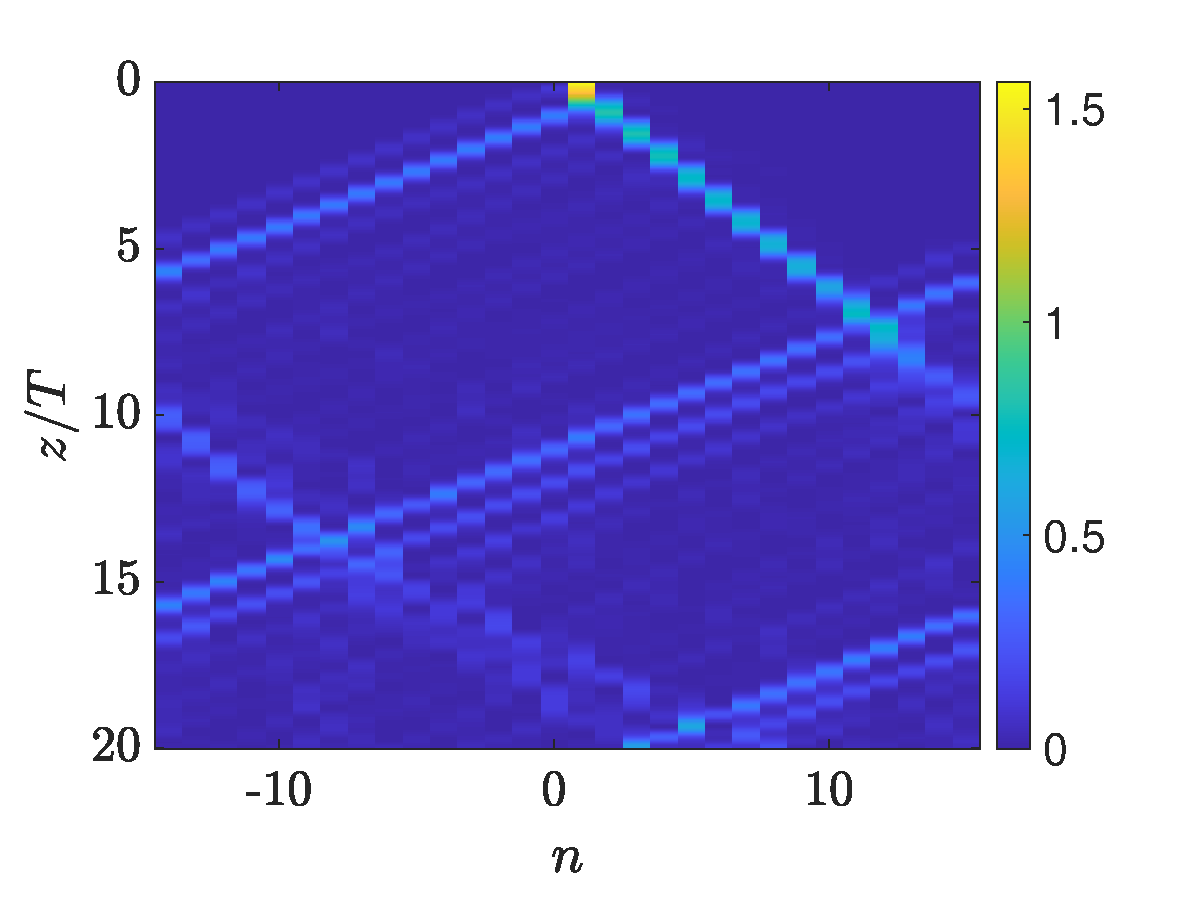
\includegraphics[width=4cm]{right125} &
    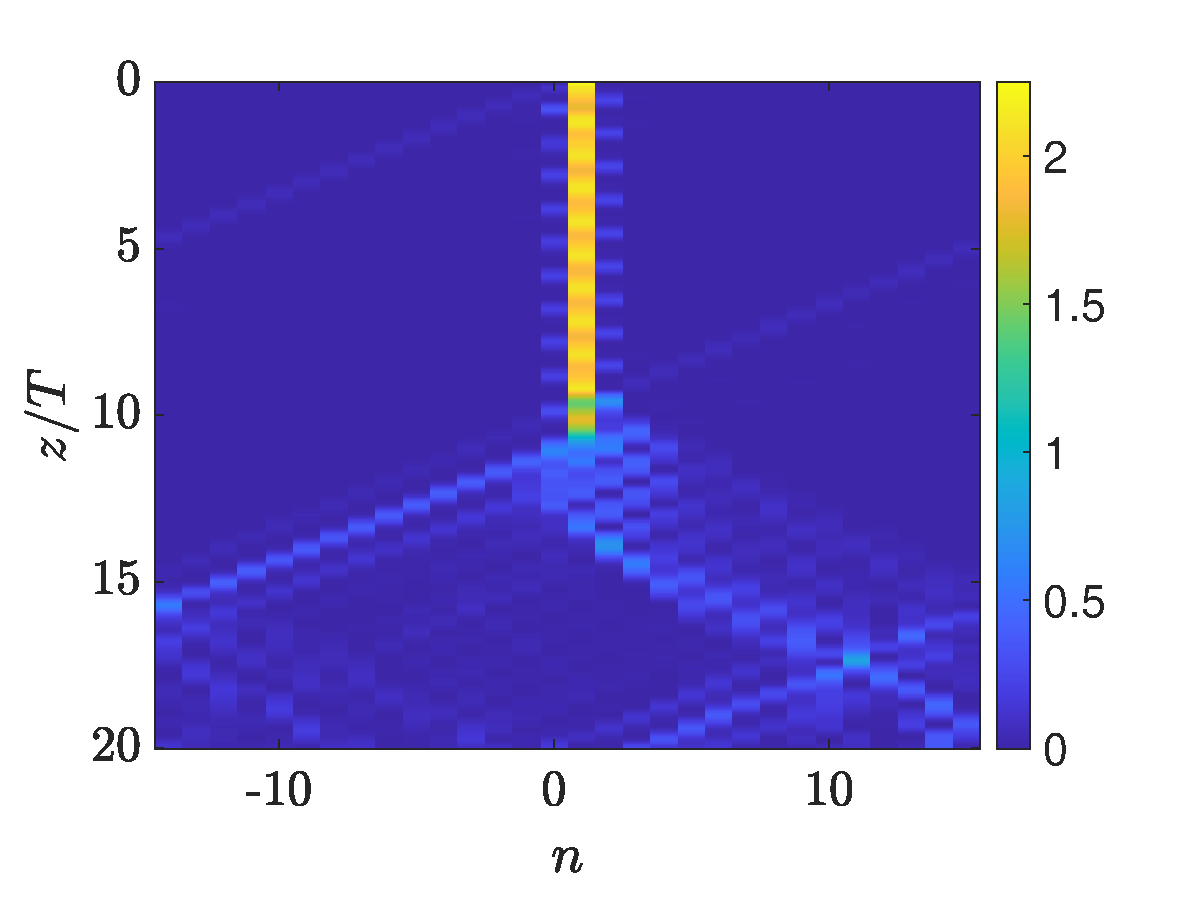
\includegraphics[width=4cm]{right15} &
    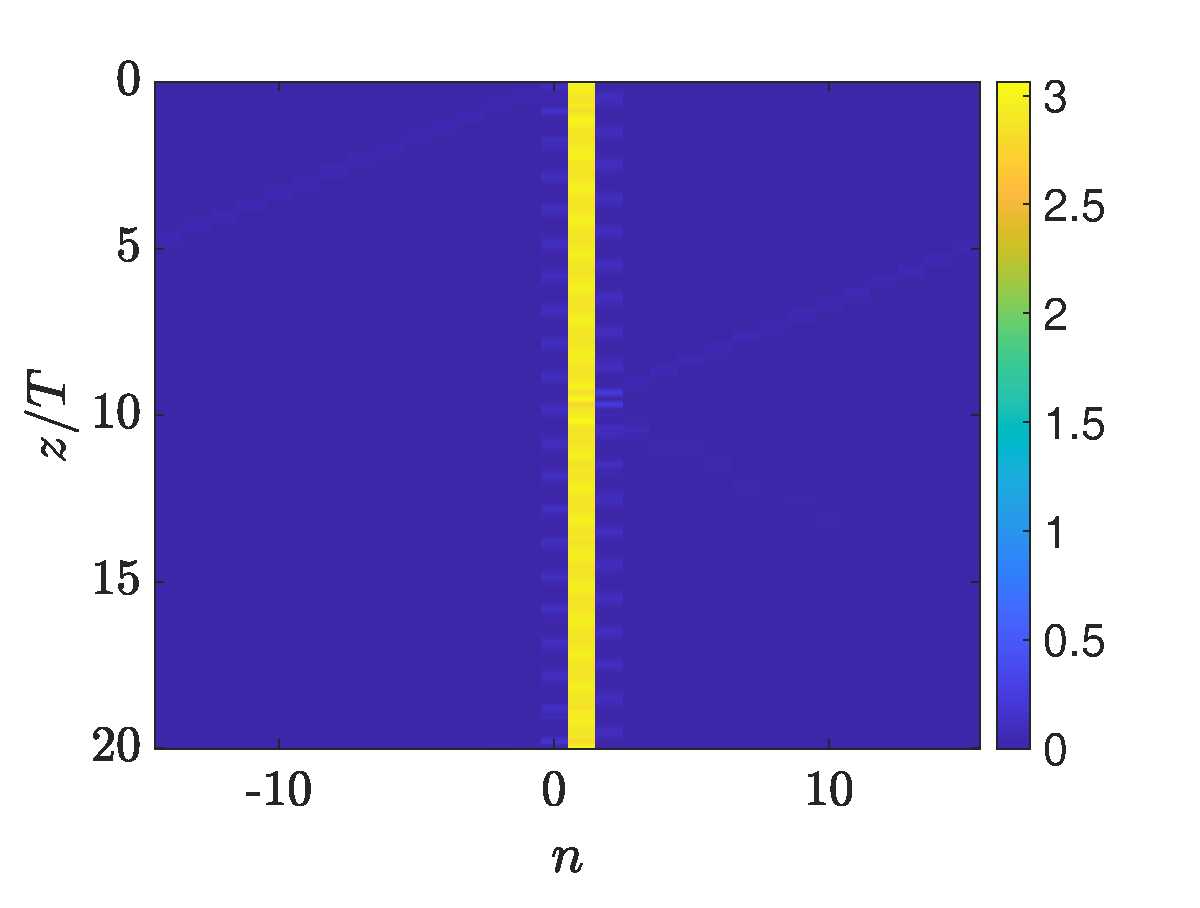
\includegraphics[width=4cm]{right175}
    \end{tabular}
    \caption{Evolution in $z$ of single-site initial condition at lattice site $n=0$ (top) and lattice site $n=1$ (bottom). Initial amplitude (left to right): 1, 1.25, 1.5, 1.75. $J_0 = 0.05$, $C=0.4$, $g=1$, 30 lattice sites. }
    \label{fig:evolmoving}
\end{figure}

\section{Coherent Structures}

Possible coherent structures that can be obtained are left-moving, right-moving, and stationary \cref{fig:coherent}. Left-moving solution moves 3 lattice sites to left in one period, reproduces itself exactly after one period. After one period, it moves one lattice site to the left, with a phase shift of $2\pi/3$). We have found two distinct right-moving solutions, both of which move 3 lattice sites to right in two periods. Note the large difference in powers between these two solutions. The lower power solution moves one lattice site to the right in 2/3 period, with a phase shift of $-2\pi/3$. The higher power solution moves one lattice to the right in 2/3 period, with no phase shift. Stationary solution reproduces itself exactly after one period. Note as well the presence of nanoptera in the moving solutions.

\begin{figure}[H]
    \centering
    \begin{tabular}{cccc}
    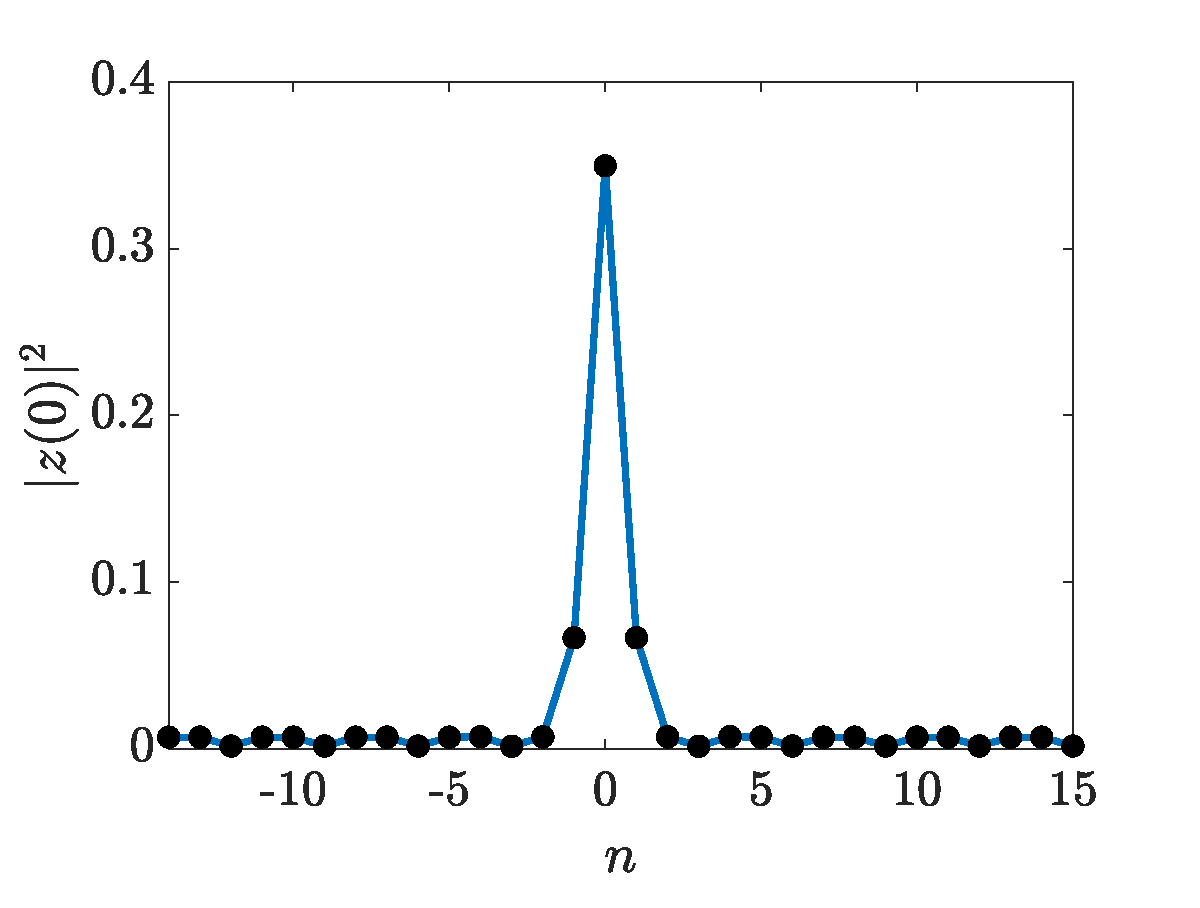
\includegraphics[width=4cm]{leftsol} &
    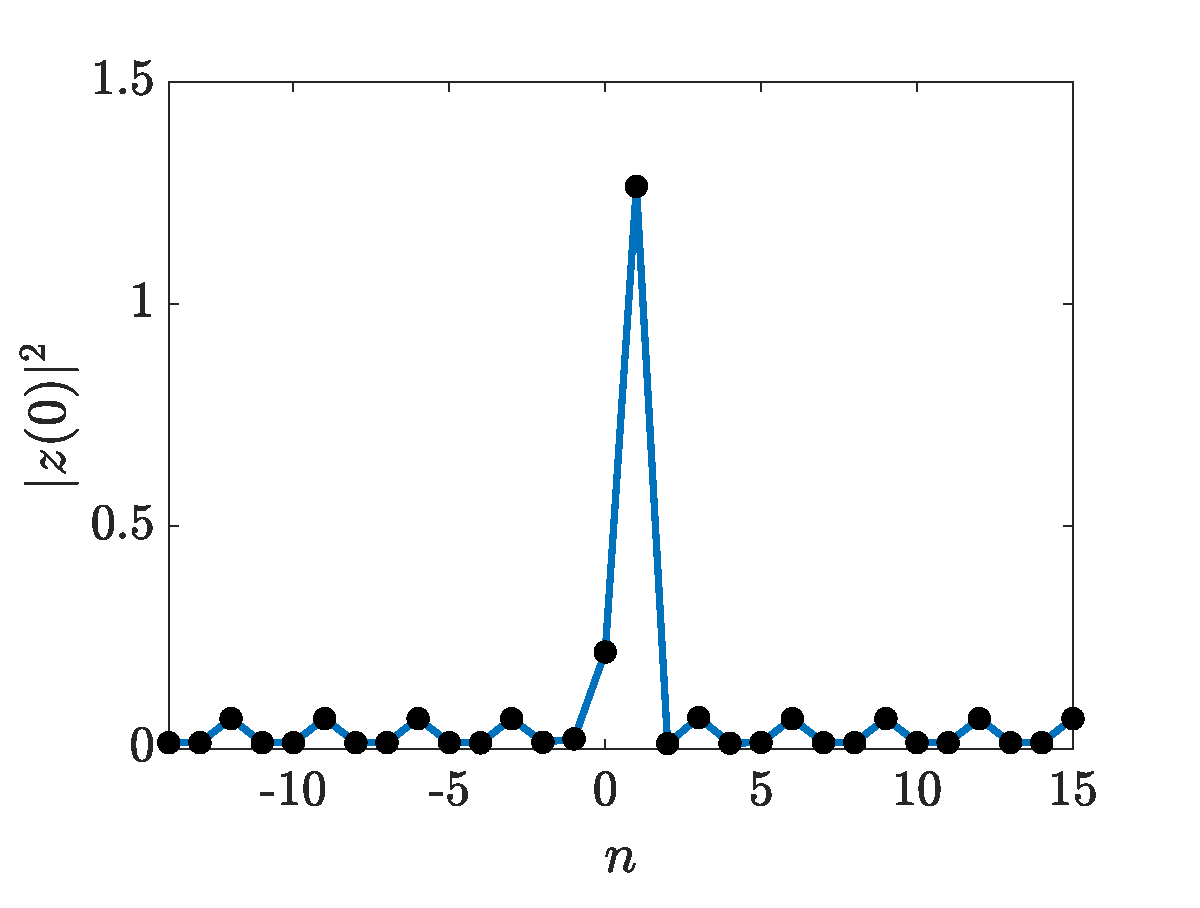
\includegraphics[width=4cm]{rightsol} &
    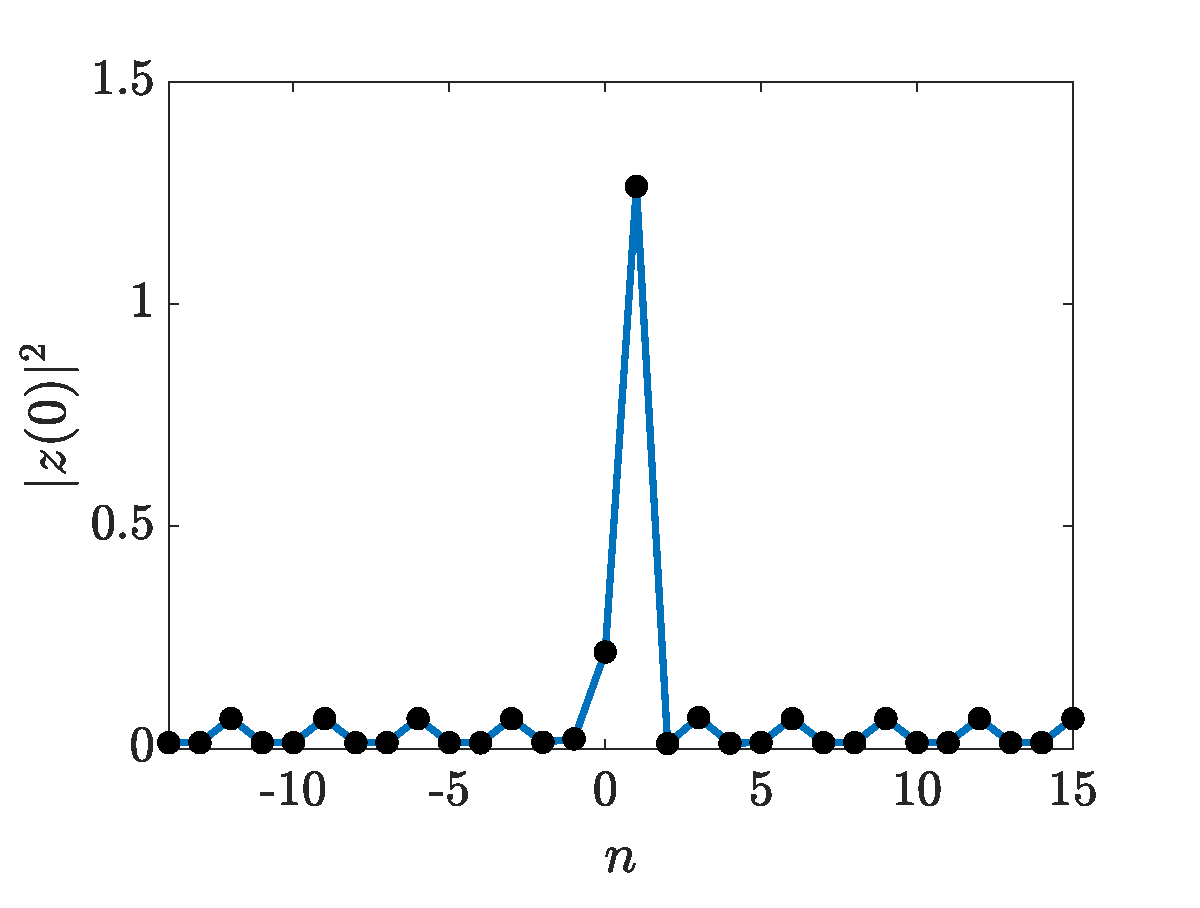
\includegraphics[width=4cm]{right0sol} &
    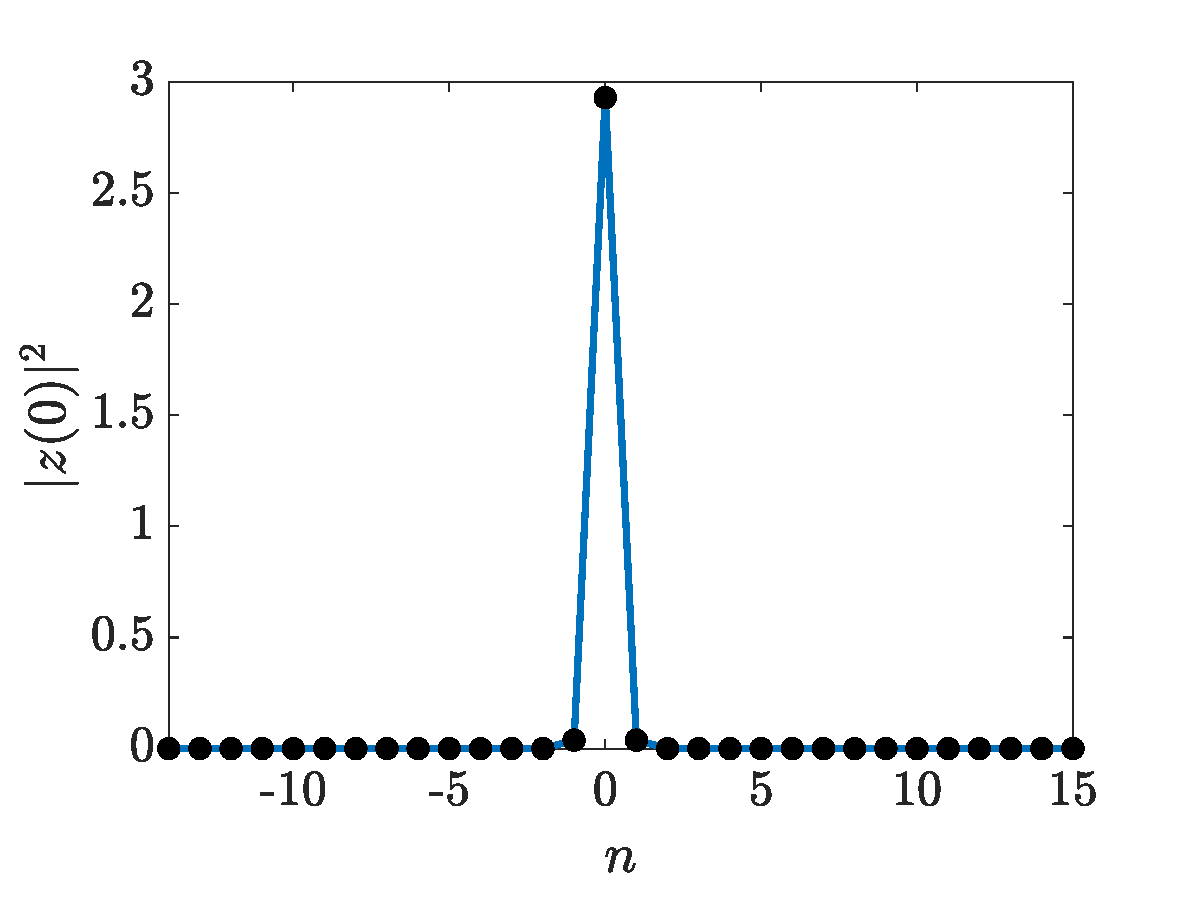
\includegraphics[width=4cm]{statsol} \\
    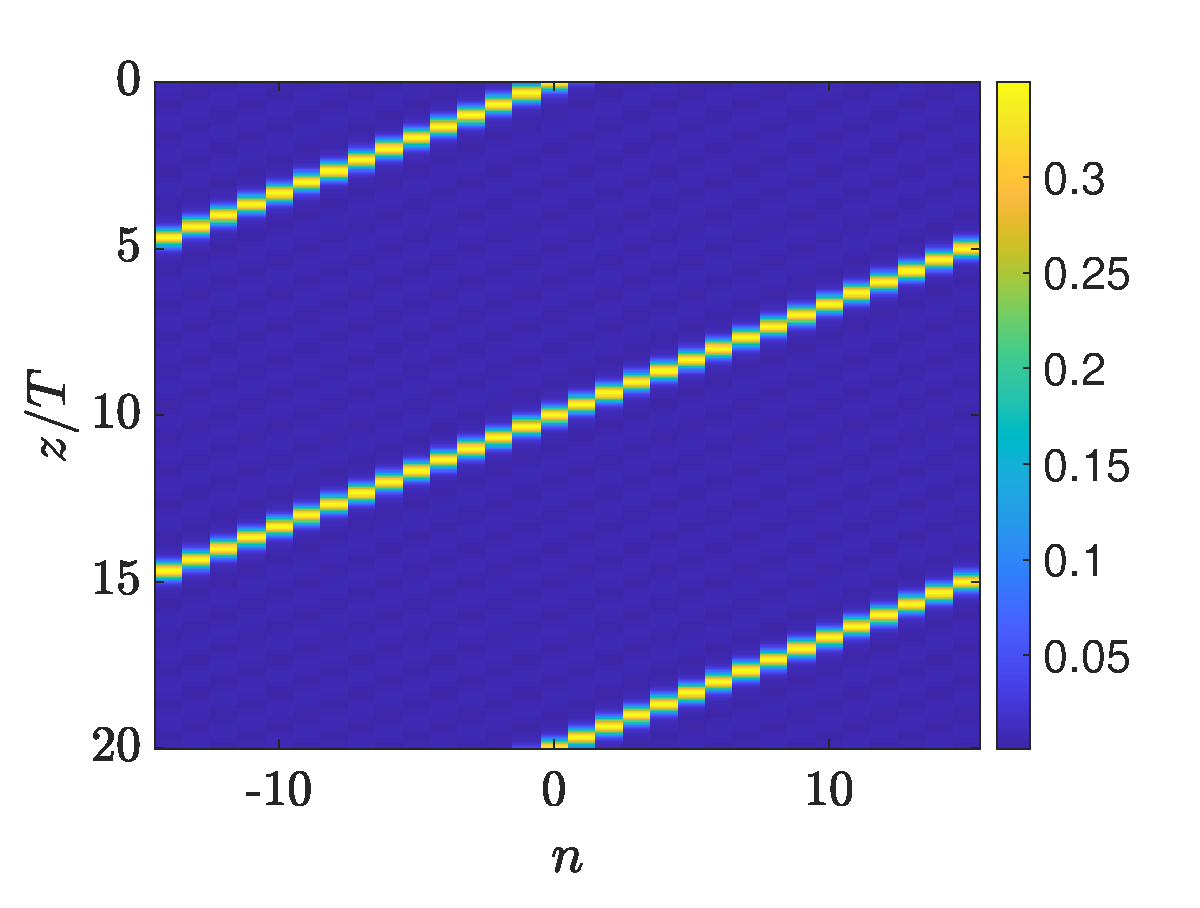
\includegraphics[width=4cm]{leftcolormap} &
    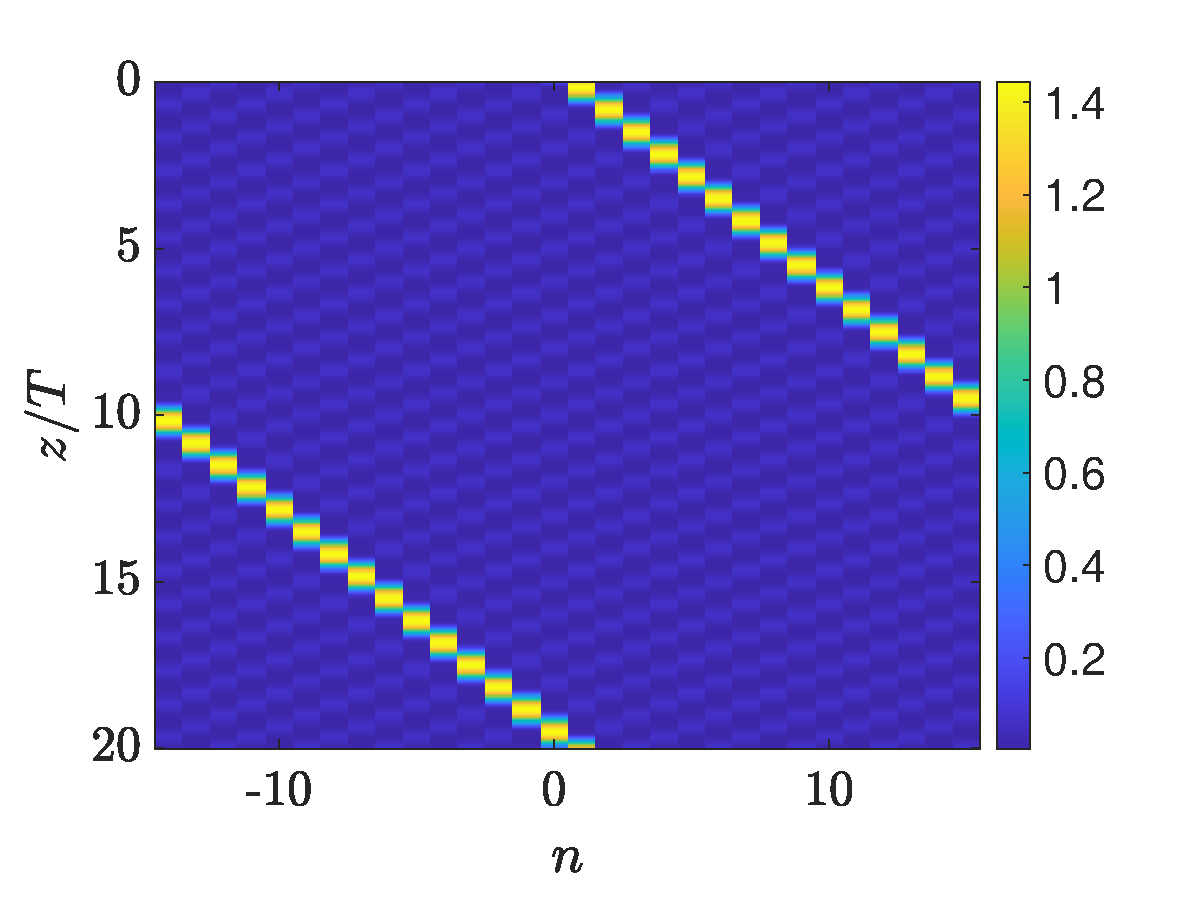
\includegraphics[width=4cm]{rightcolormap} &
    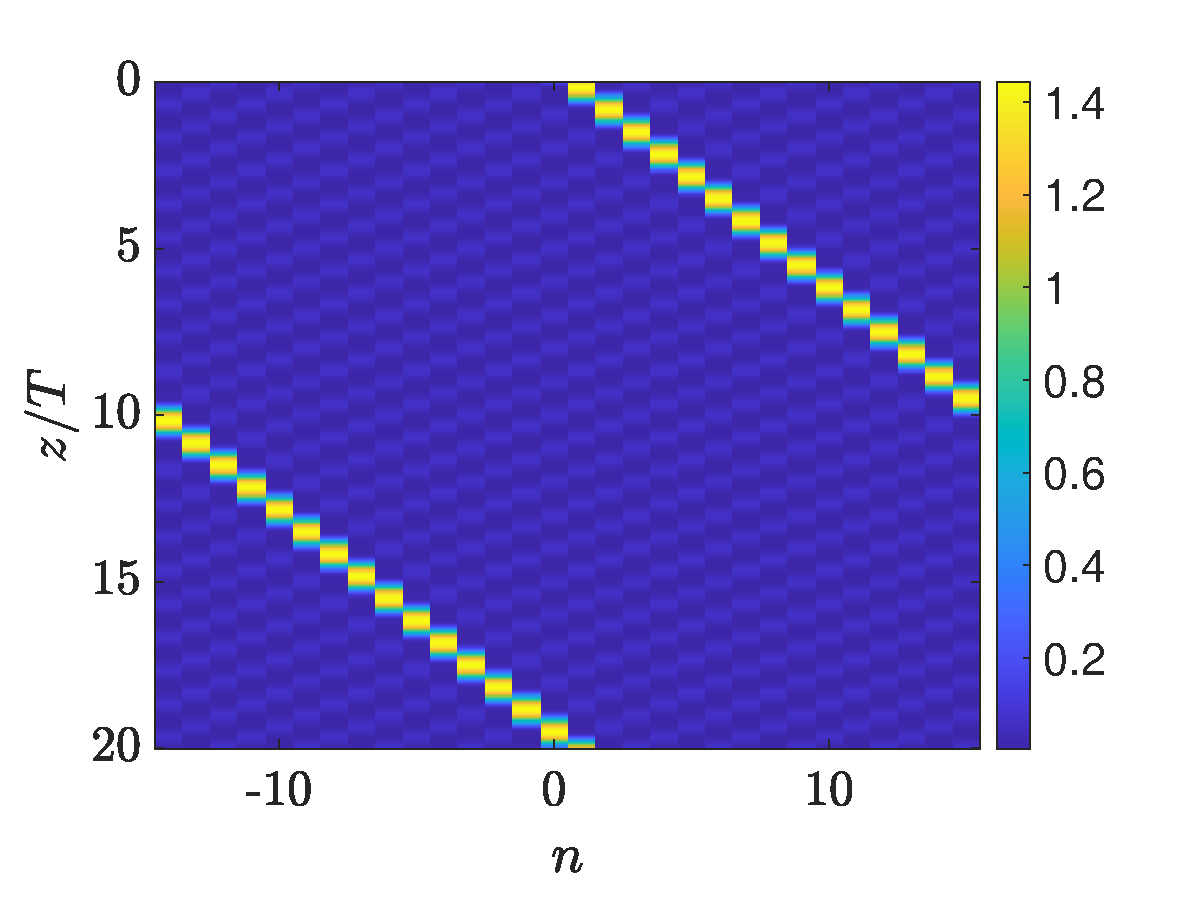
\includegraphics[width=4cm]{right0colormap} &
    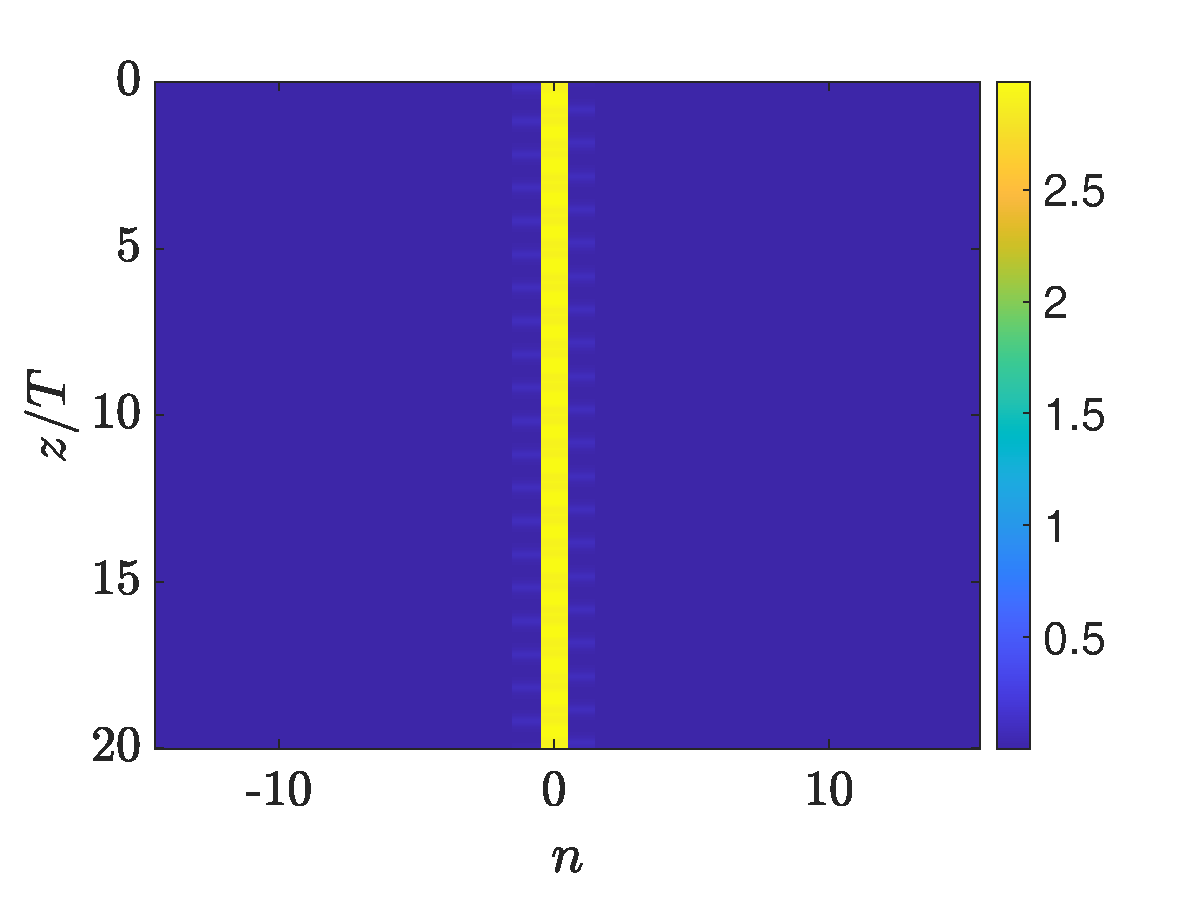
\includegraphics[width=4cm]{statcolormap} 
    \end{tabular}
    \caption{Left-moving, right-moving (lower power), right-moving (higher power), and stationary coherent structures. Top is power of solution at $z=0$, bottom is colormap showing evolution of solution in $z$. $J_0 = 0.05$, $C=0.4$, $g=1$, 30 lattice sites.}
    \label{fig:coherent}
\end{figure}

\section{Parameter continuation}

Parameter continuation in $C$ can be performed on these solutions. Note that for the left-moving and lower power right-moving solution, there is a critical value of $C$ at which the nanoptera disappear. This value is different for these two solutions. This does not occur for the high-power right-moving solution.

\begin{figure}[H]
    \centering
    \begin{tabular}{ccc}
    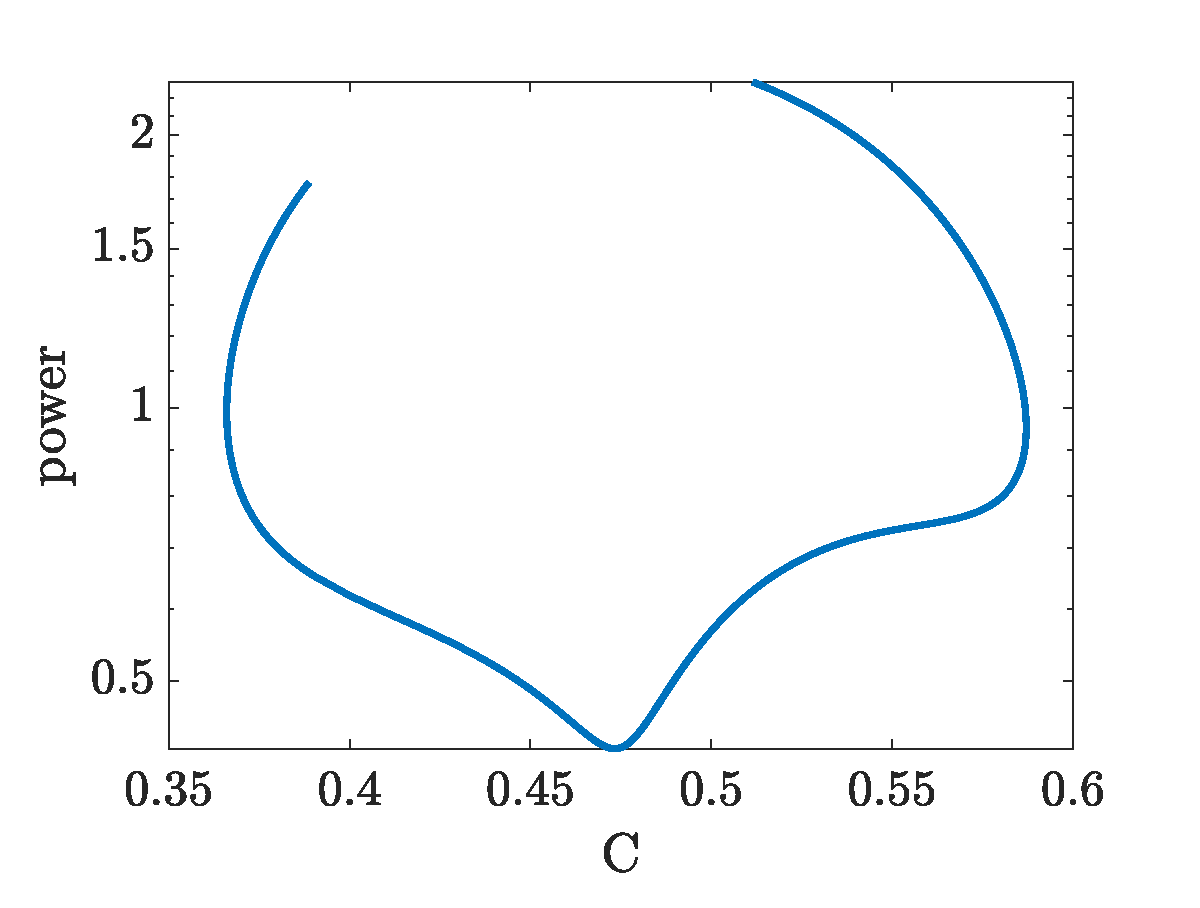
\includegraphics[width=5cm]{leftcontpower}   &
    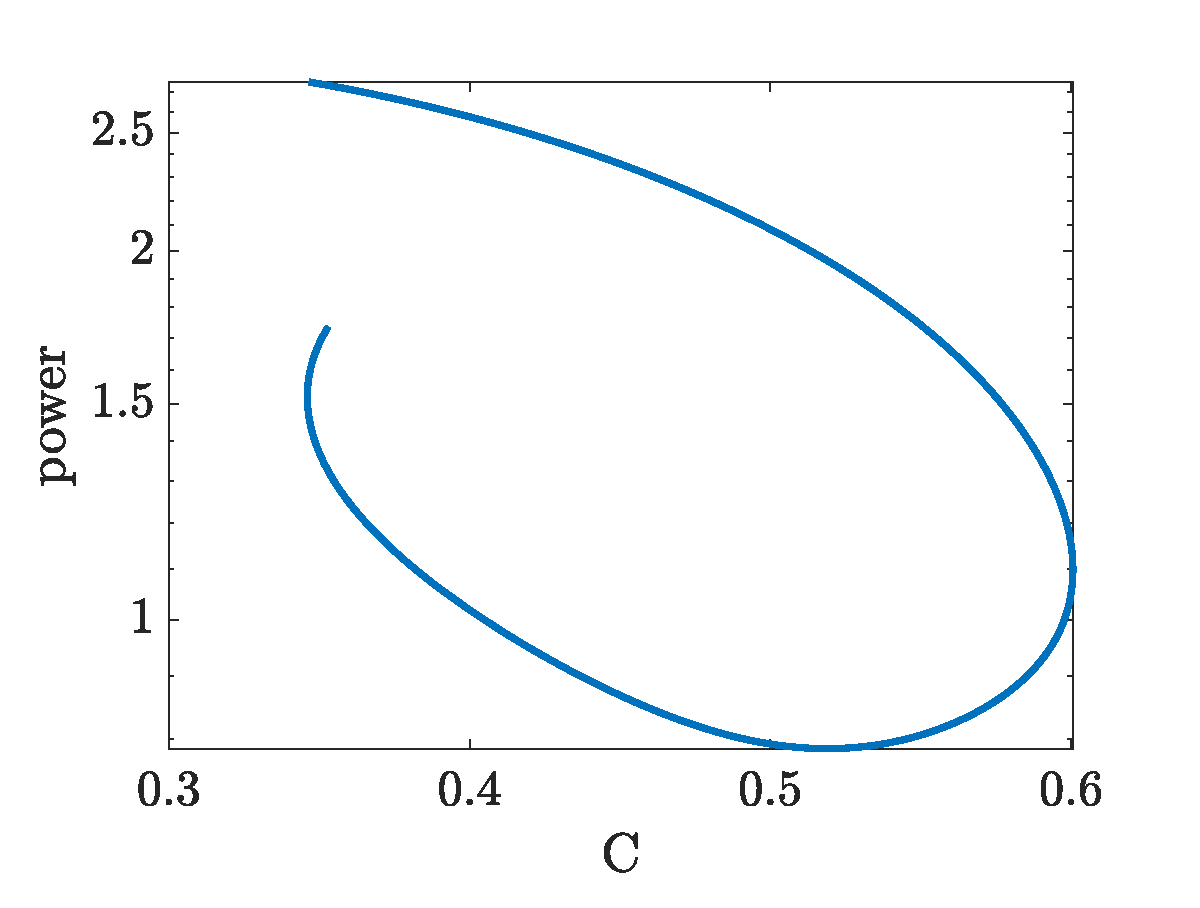
\includegraphics[width=5cm]{rightcontpower}  &
    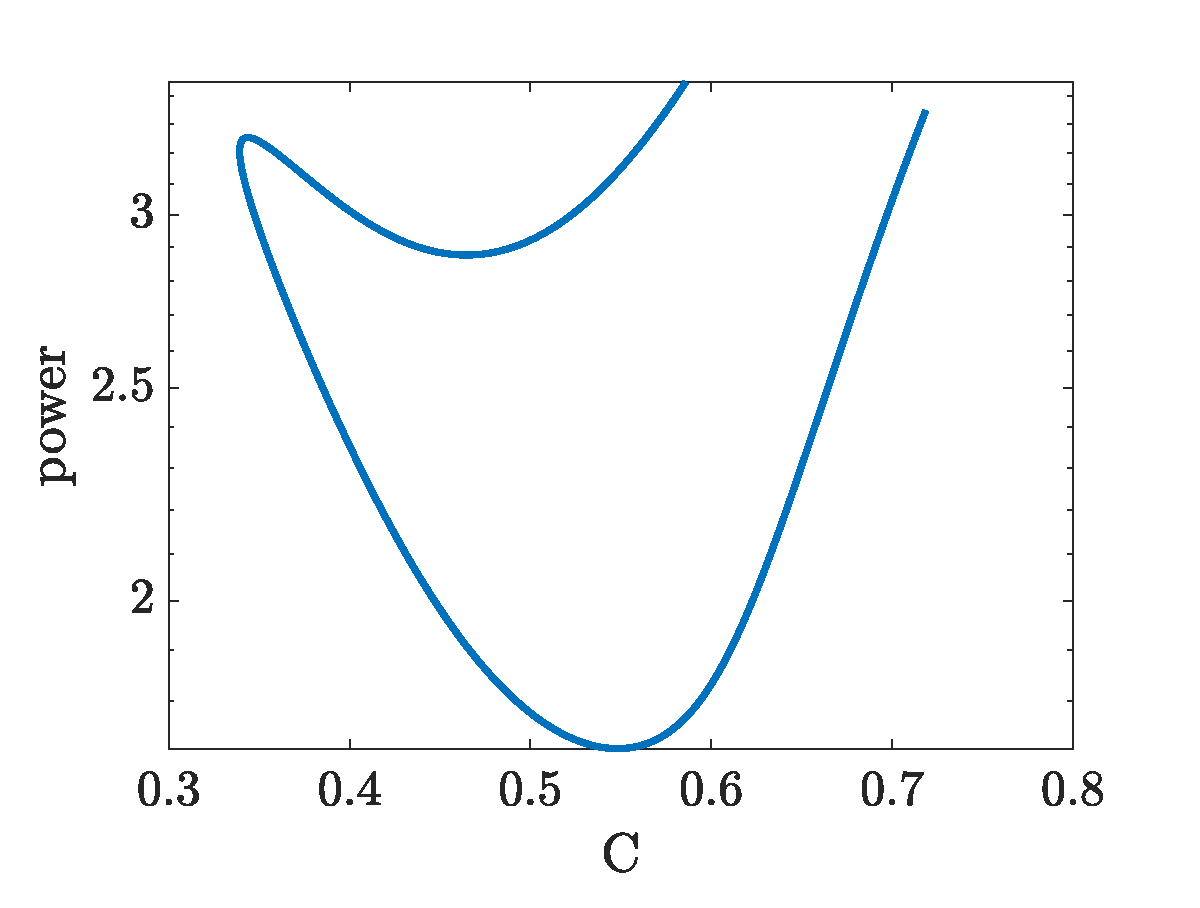
\includegraphics[width=5cm]{right0contpower} \\
    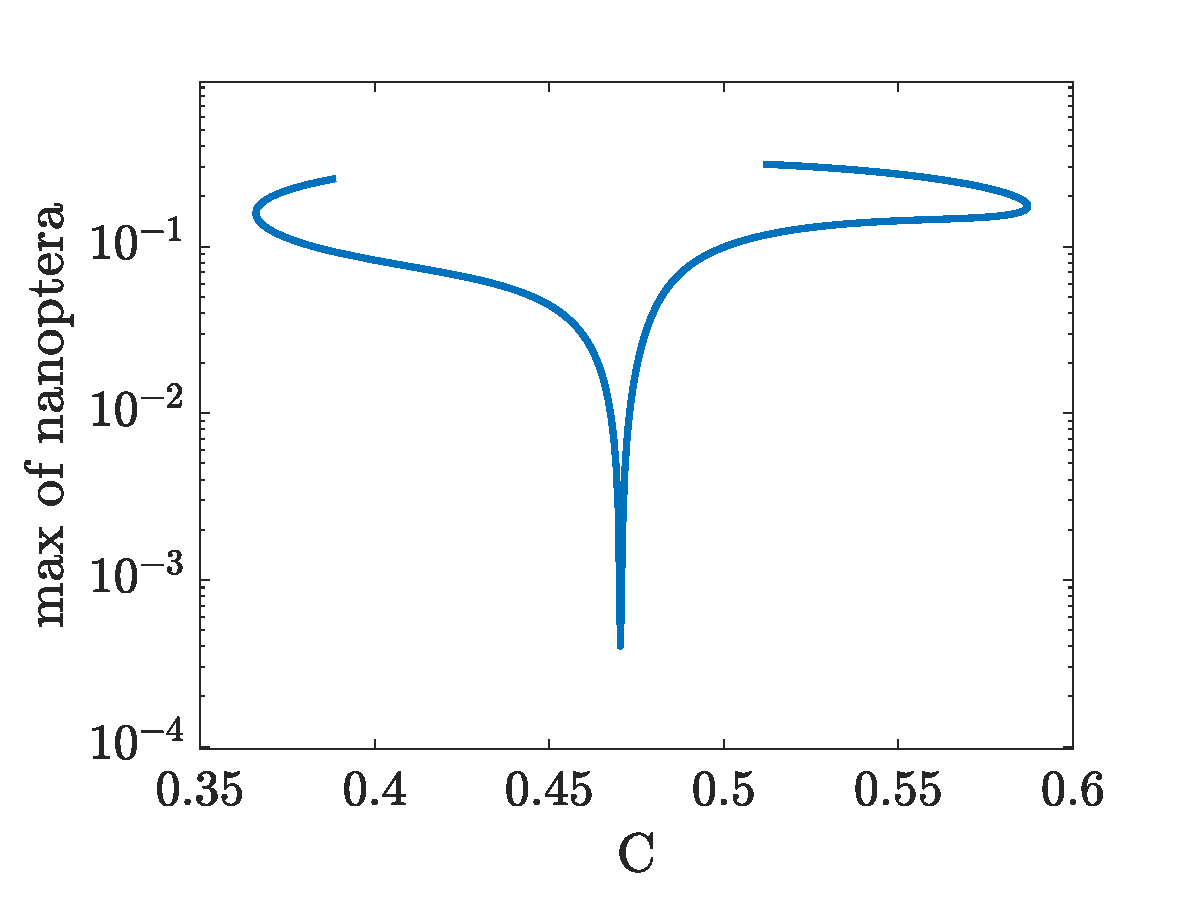
\includegraphics[width=5cm]{leftcontnanop}   &
    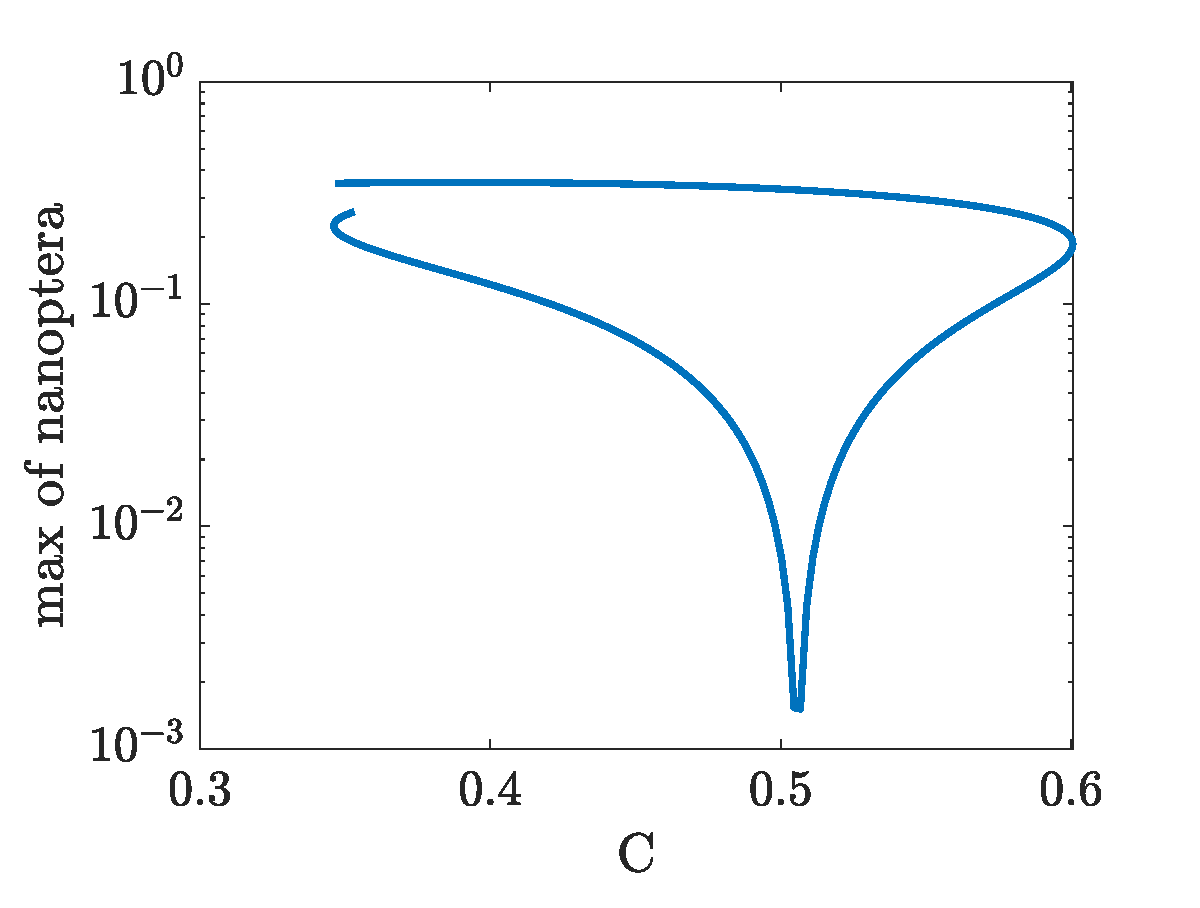
\includegraphics[width=5cm]{rightcontnanop}  &
    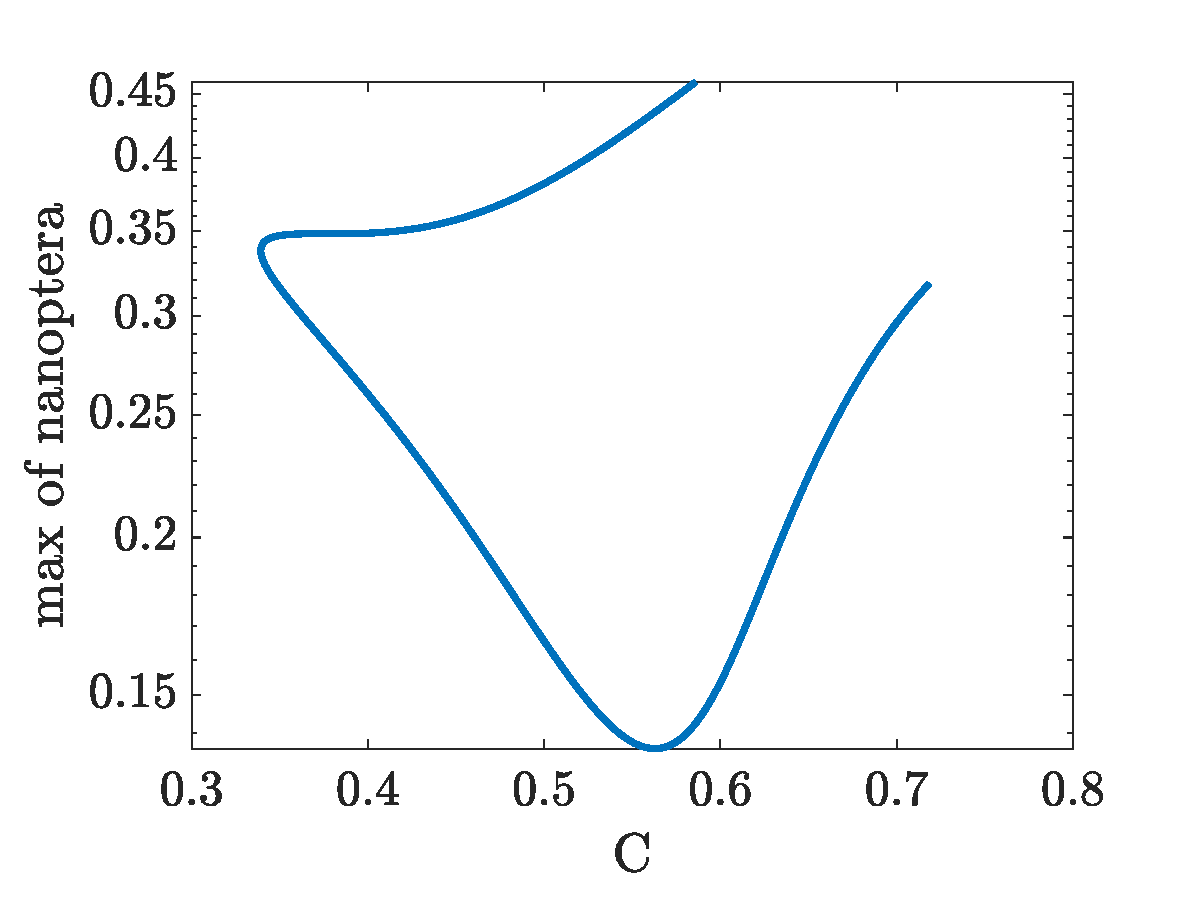
\includegraphics[width=5cm]{right0contnanop} 
    \end{tabular}
    \caption{Continuation in $C$ for left-moving, right-moving (lower power), and right-moving (higher power) solutions. Top plot is power of solution vs $C$, bottom is max of nanoptera vs $C$. $J_0 = 0.05$, $g=1$, 30 lattice sites.}
    \label{fig:cont}
\end{figure}

\section{Left moving solution}

\begin{figure}[H]
    \centering
    \begin{tabular}{ccc}
    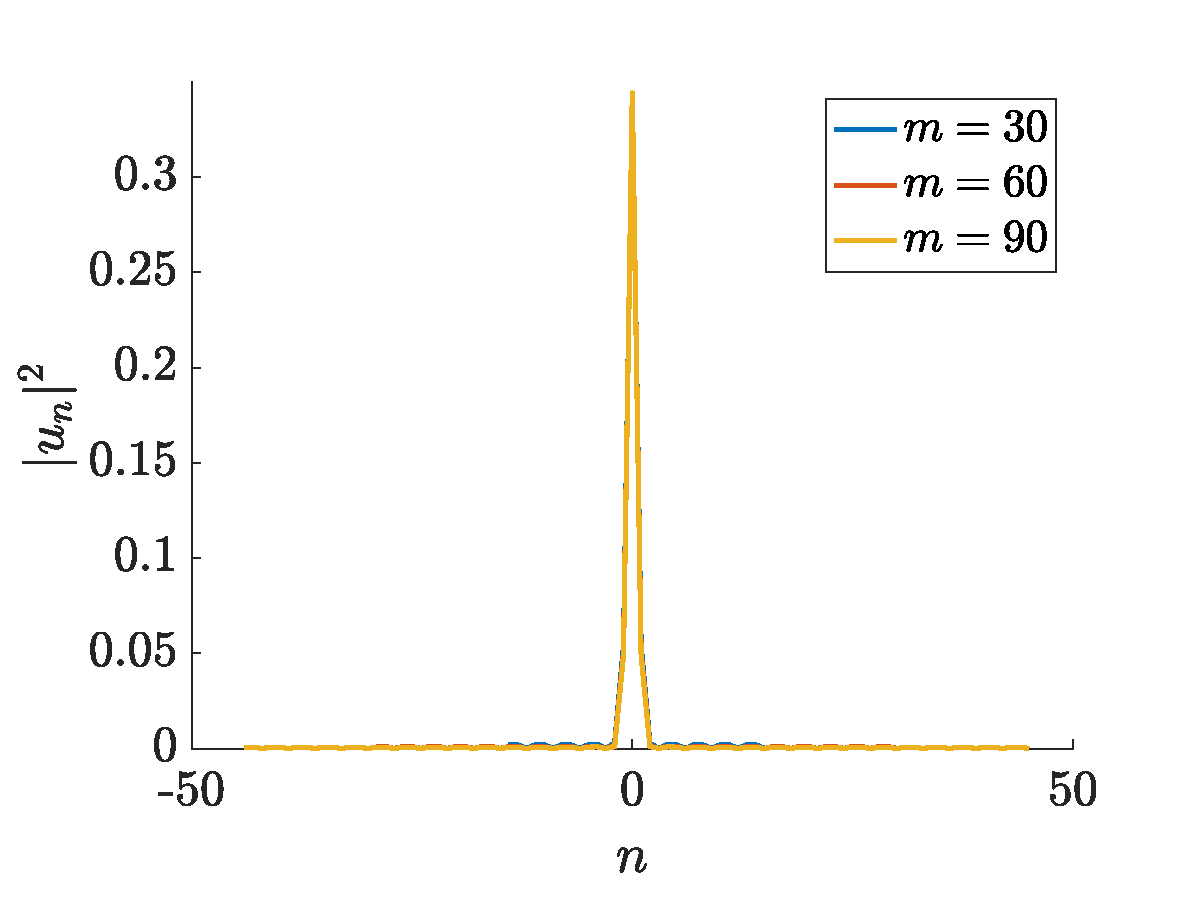
\includegraphics[width=5cm]{leftm} &
    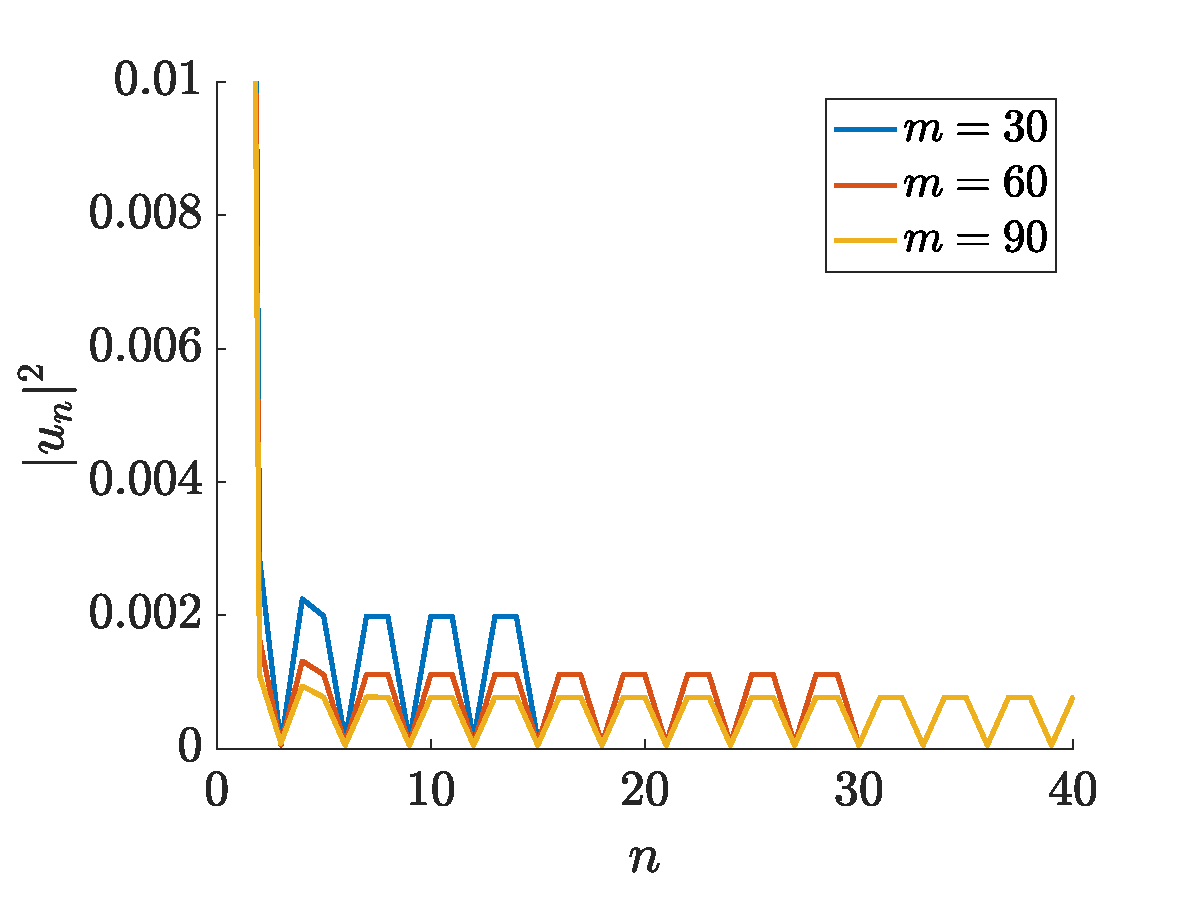
\includegraphics[width=5cm]{leftmnanop} &
    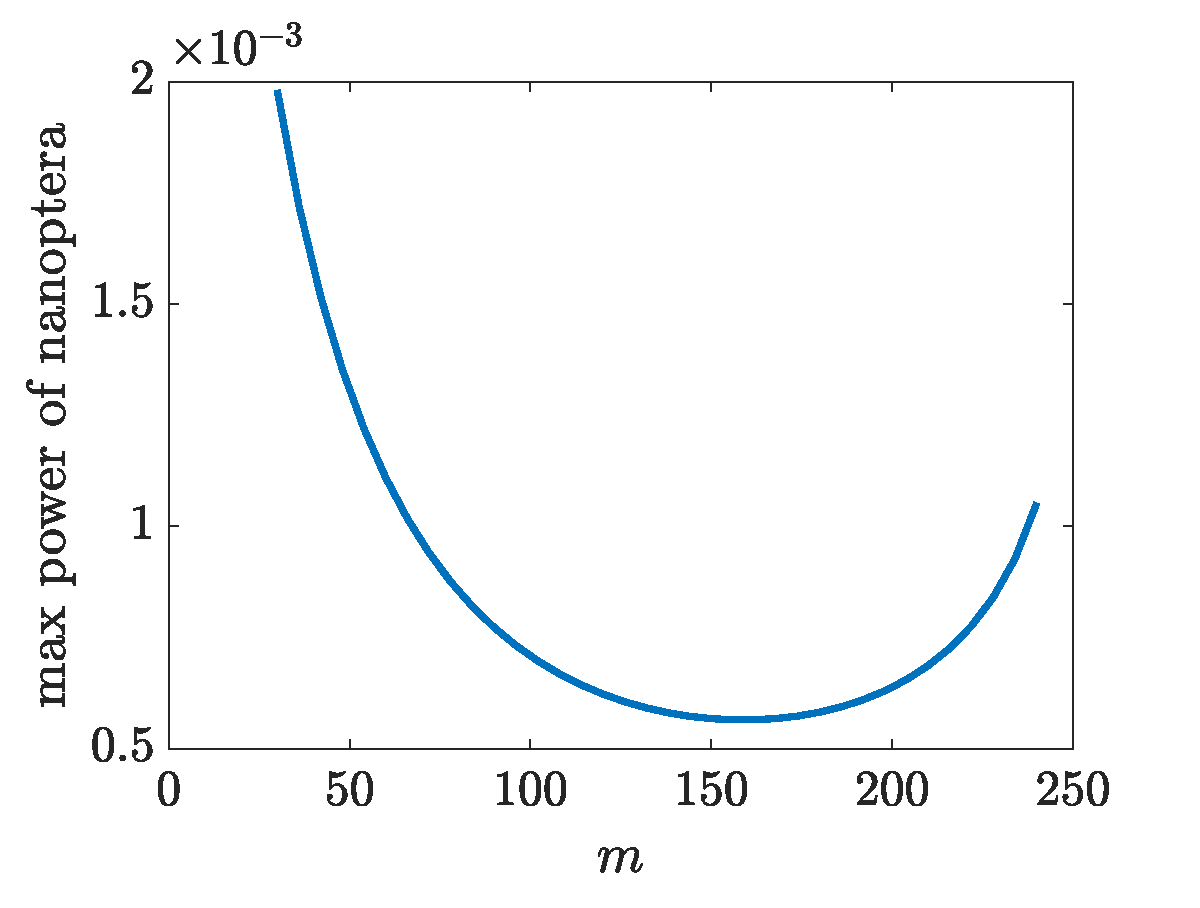
\includegraphics[width=5cm]{leftnanopmax} \\
    \end{tabular}
    \caption{Left-moving solution for three values of $m$ (left), zoom on nanoptera tails of these solutions (center), max power of nanoptera vs $m$ (right). $J_0 = 0.05$, $C = 0.45$, $g=1$.}
    \label{fig:left1}
\end{figure}

\begin{figure}[H]
    \centering
    \begin{tabular}{ccc}
    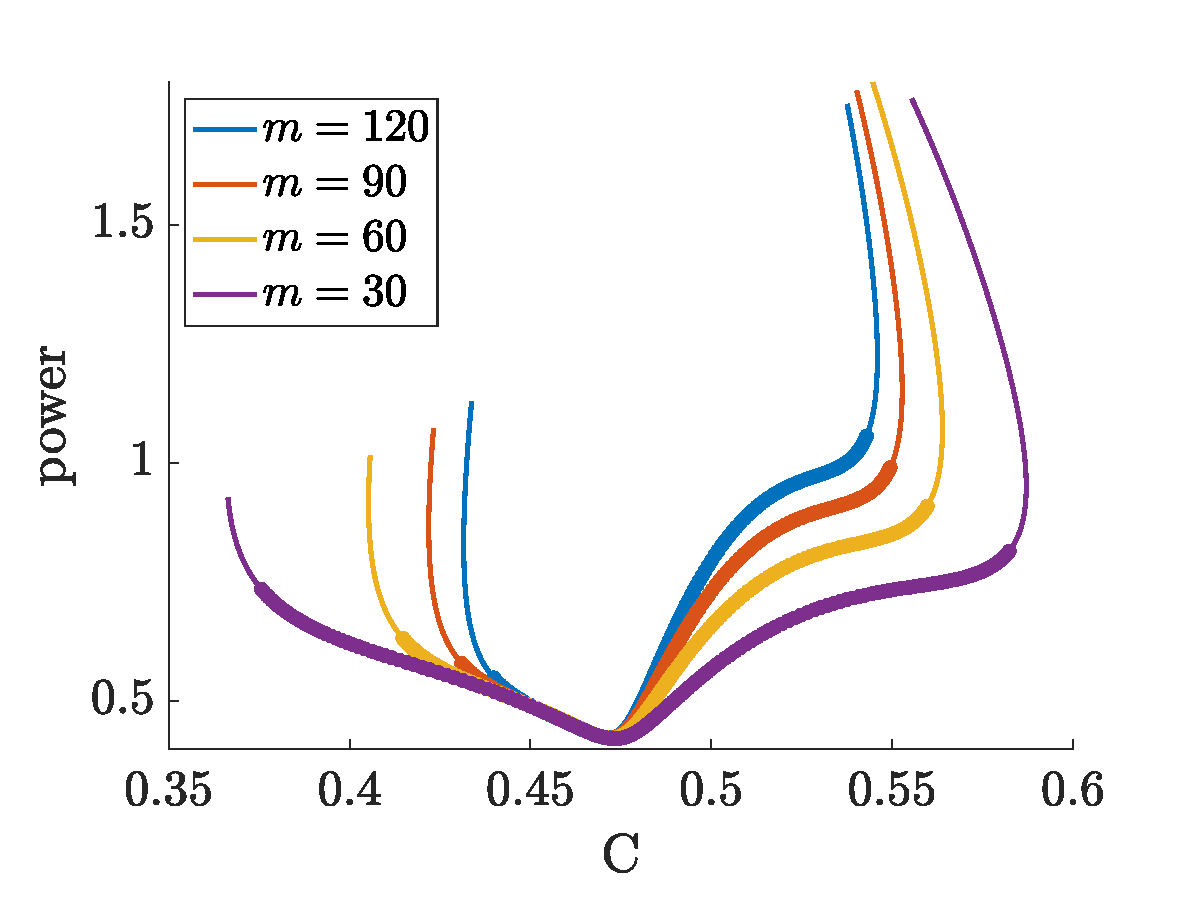
\includegraphics[width=5cm]{leftBD1} &
    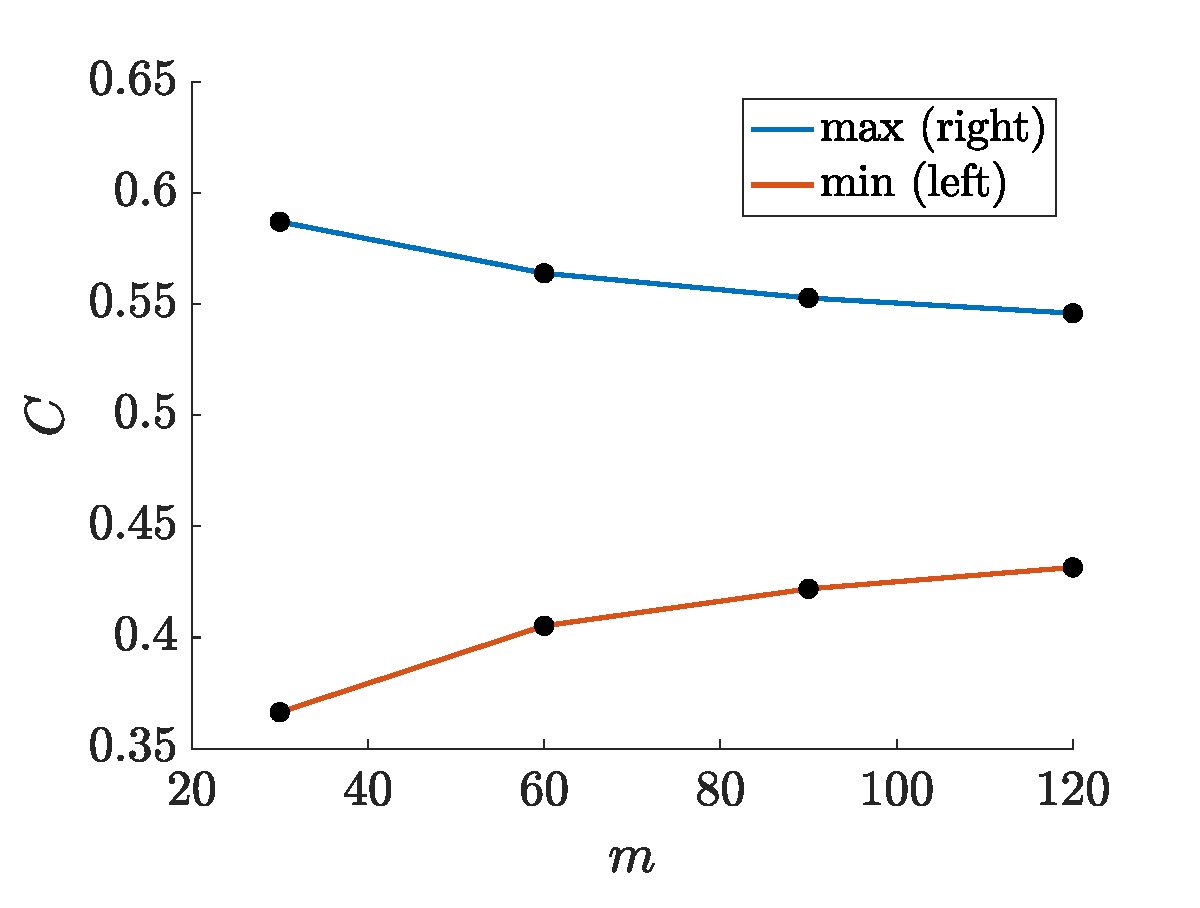
\includegraphics[width=5cm]{leftmaxminC} 
    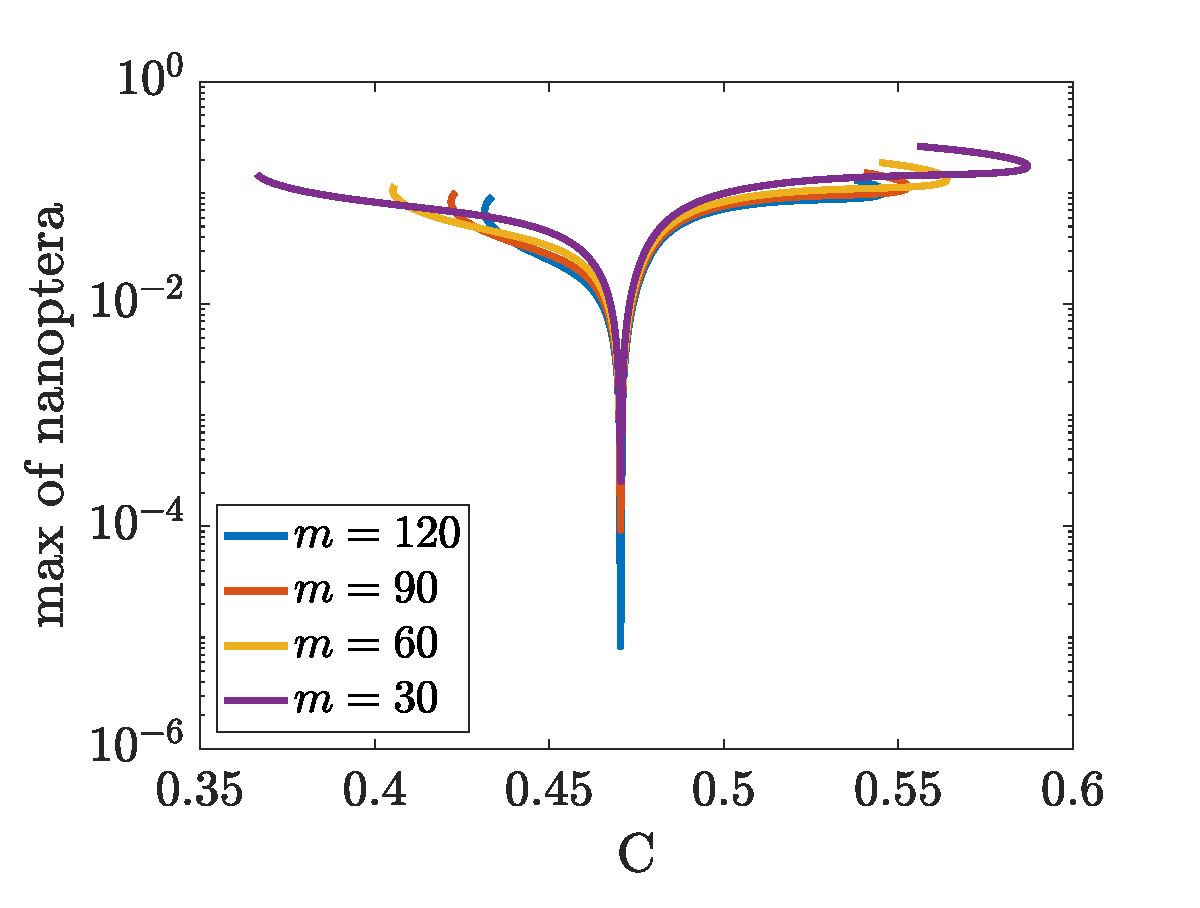
\includegraphics[width=5cm]{leftBDnanop} 
    \end{tabular}
    \caption{Left: Bifurcation diagram for continuation in $C$ for different lattice sizes $m$. Spectrally stable portion is thicker line. Spectral stability here is defined by having no purely real Floquet multipliers greater than 1. Multipliers off of the unit circle resulting from band collisions are not counted (these are essentially always present). For all values of $m$, spectral instability results from a collision of Floquet multipliers on unit circle at $(1,0)$, which leads to a real eigenvalue greater than 1. This occurs for both the right and left instabilities on the bifurcation diagram. See figures below for Floquet spectrum and form of corresponding eigenfunction.
    Center: max and min of $C$ on bifurcation diagram for varying $m$. 
    Right: max of nanoptera vs. $C$.}
    \label{fig:left2}
\end{figure}

\begin{figure}[H]
    \centering
    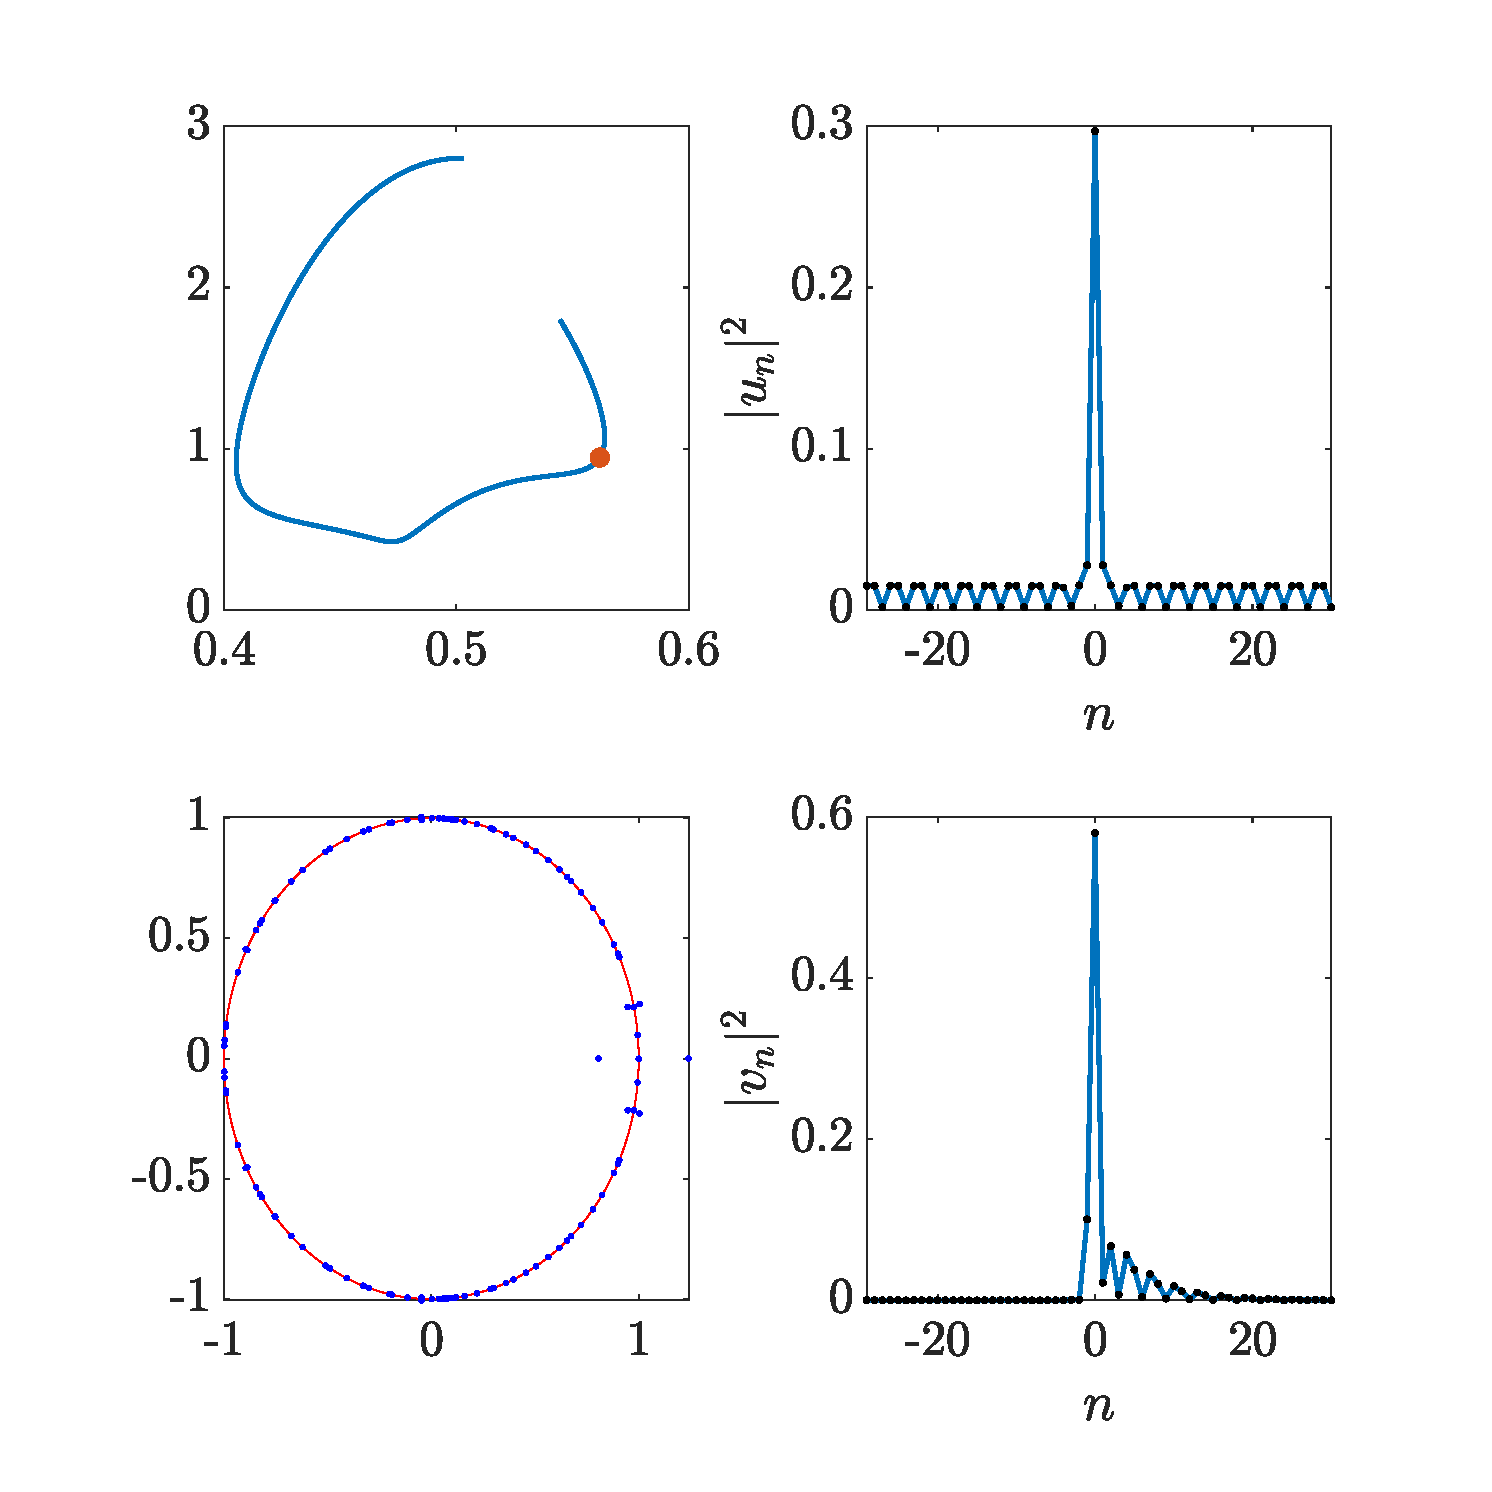
\includegraphics[width=12cm]{leftafterinstabilityR}
    \caption{Solution after the instability on right of bifurcation diagram for $m=60$ (top right). Position on bifurcation diagram shown in top left. Floquet spectrum in bottom left. Corresponding eigenfunction to real eigenvalue is localized (bottom right). $C = 0.5618$}
    \label{fig:leftinstabR}
\end{figure}

\begin{figure}[H]
    \centering
    \begin{tabular}{cc}
    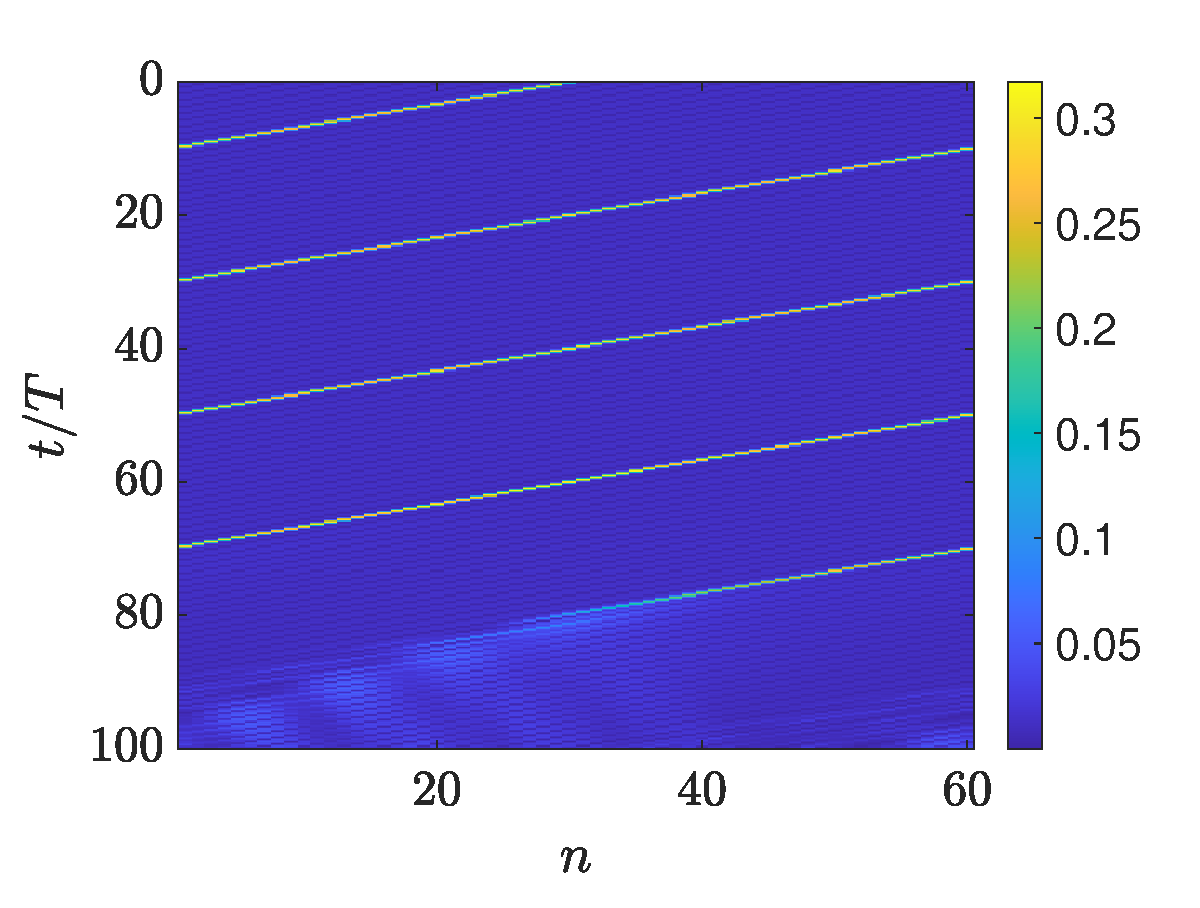
\includegraphics[width=7cm]{leftafterinstabilityRtimestep} &
    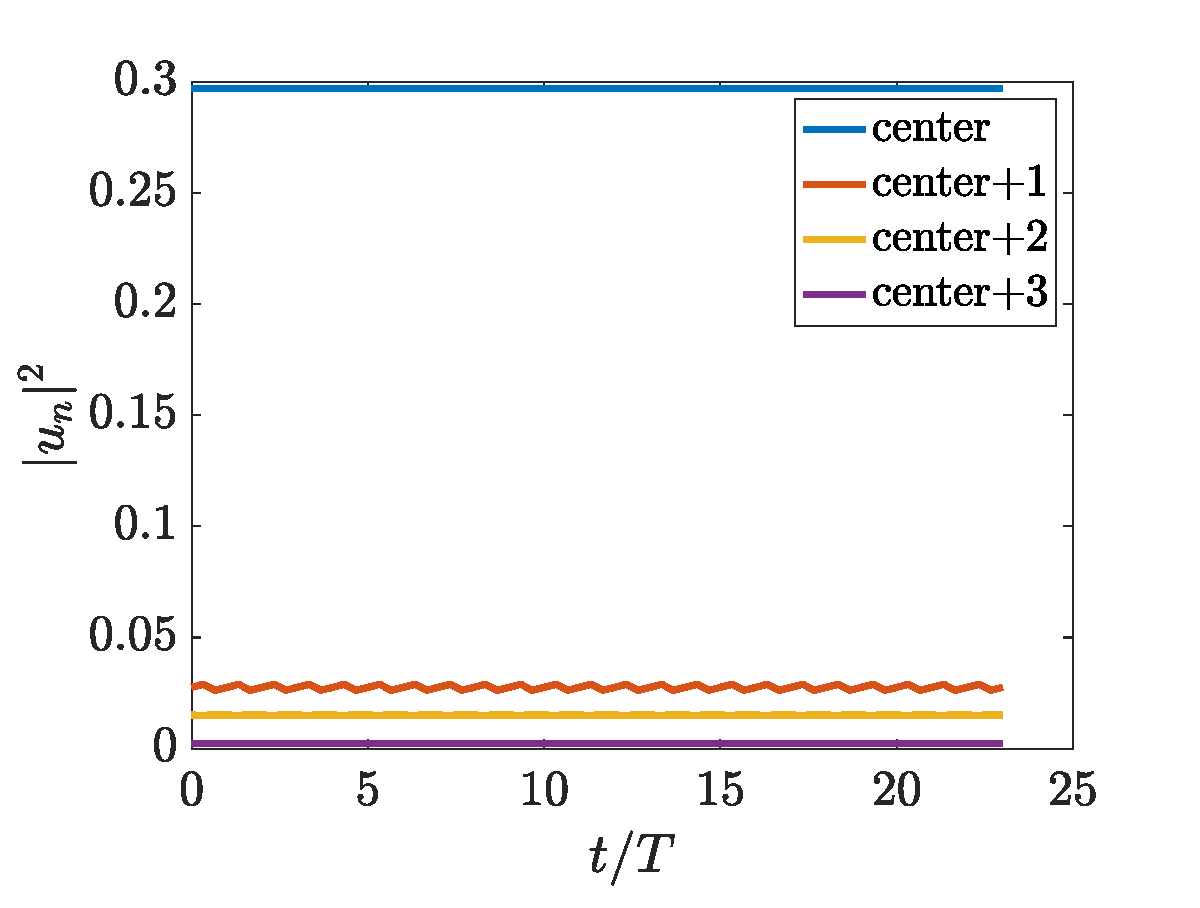
\includegraphics[width=7cm]{leftafterinstabilityRpower} \\ 
    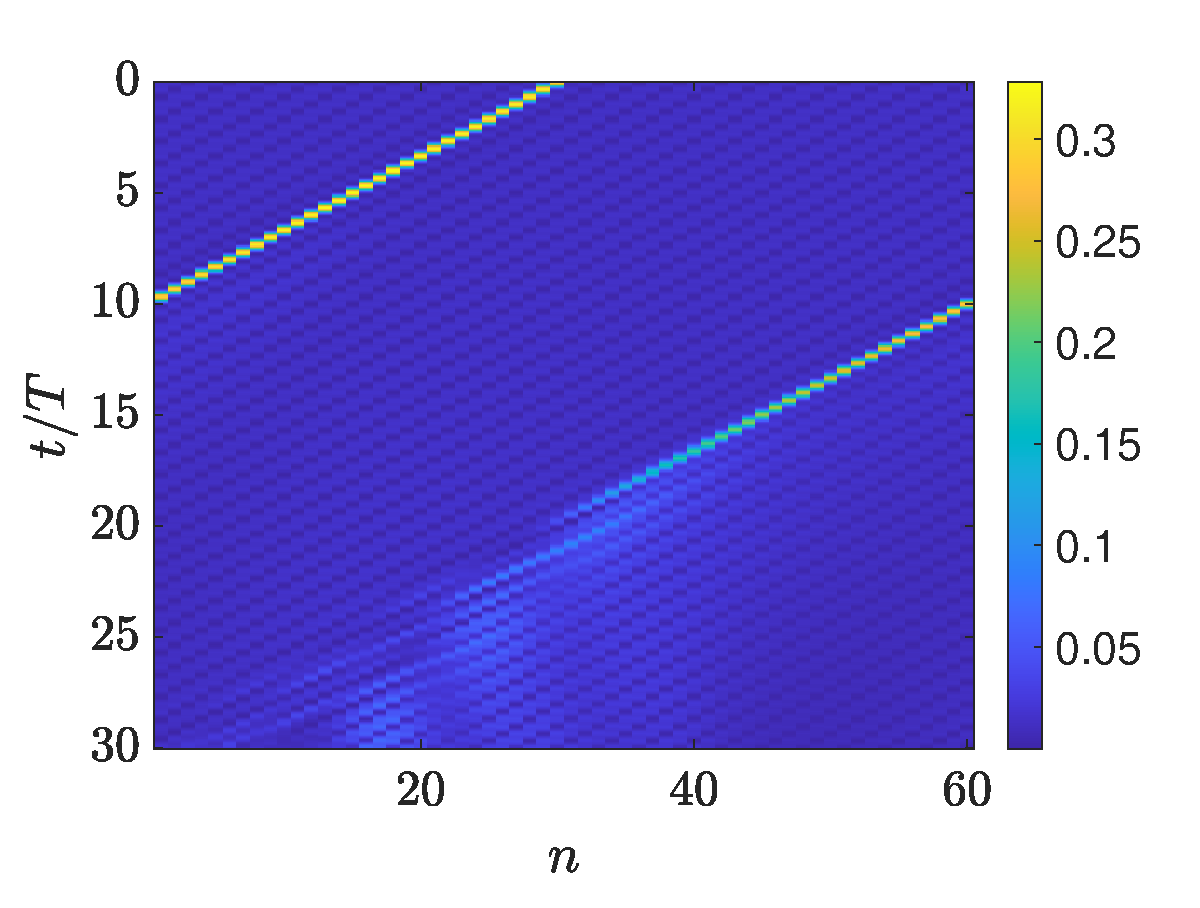
\includegraphics[width=7cm]{leftafterinstabilityRperttimestep} &
    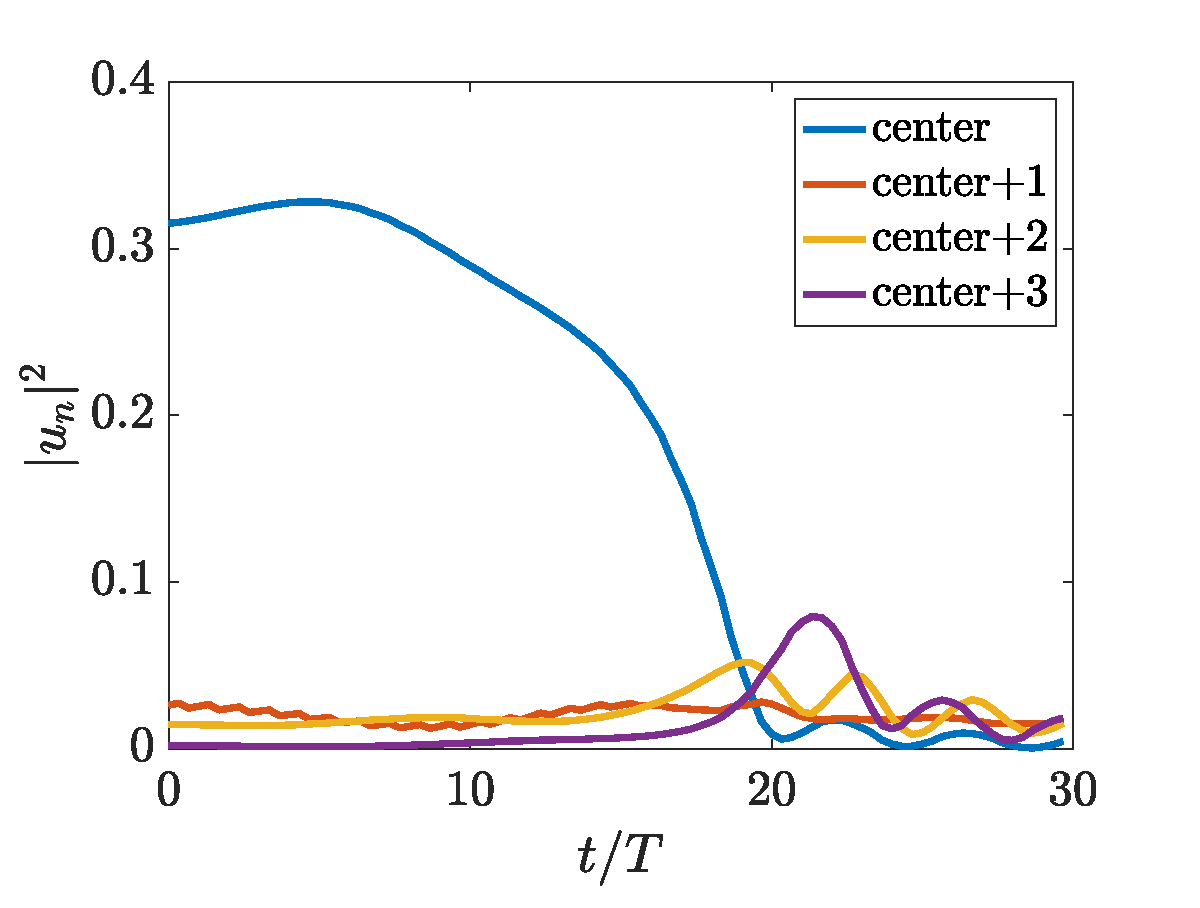
\includegraphics[width=7cm]{leftafterinstabilityRpertpower}
    \end{tabular}
    \caption{Colormap showing time evolution of $|u_n|^2$ (left) and power of center site and right neighbors of left-moving solution for solution after the instability on right of bifurcation diagram for $m=60$. Top is unperturbed solution, bottom is perturbed by adding $\delta$ times the eigenfunction corresponding to the unstable, real Floquet eigenmode. $\delta = 0.1$, $C=0.5618$. }
    \label{fig:leftinstabRpert}
\end{figure}

\begin{figure}[H]
    \centering
    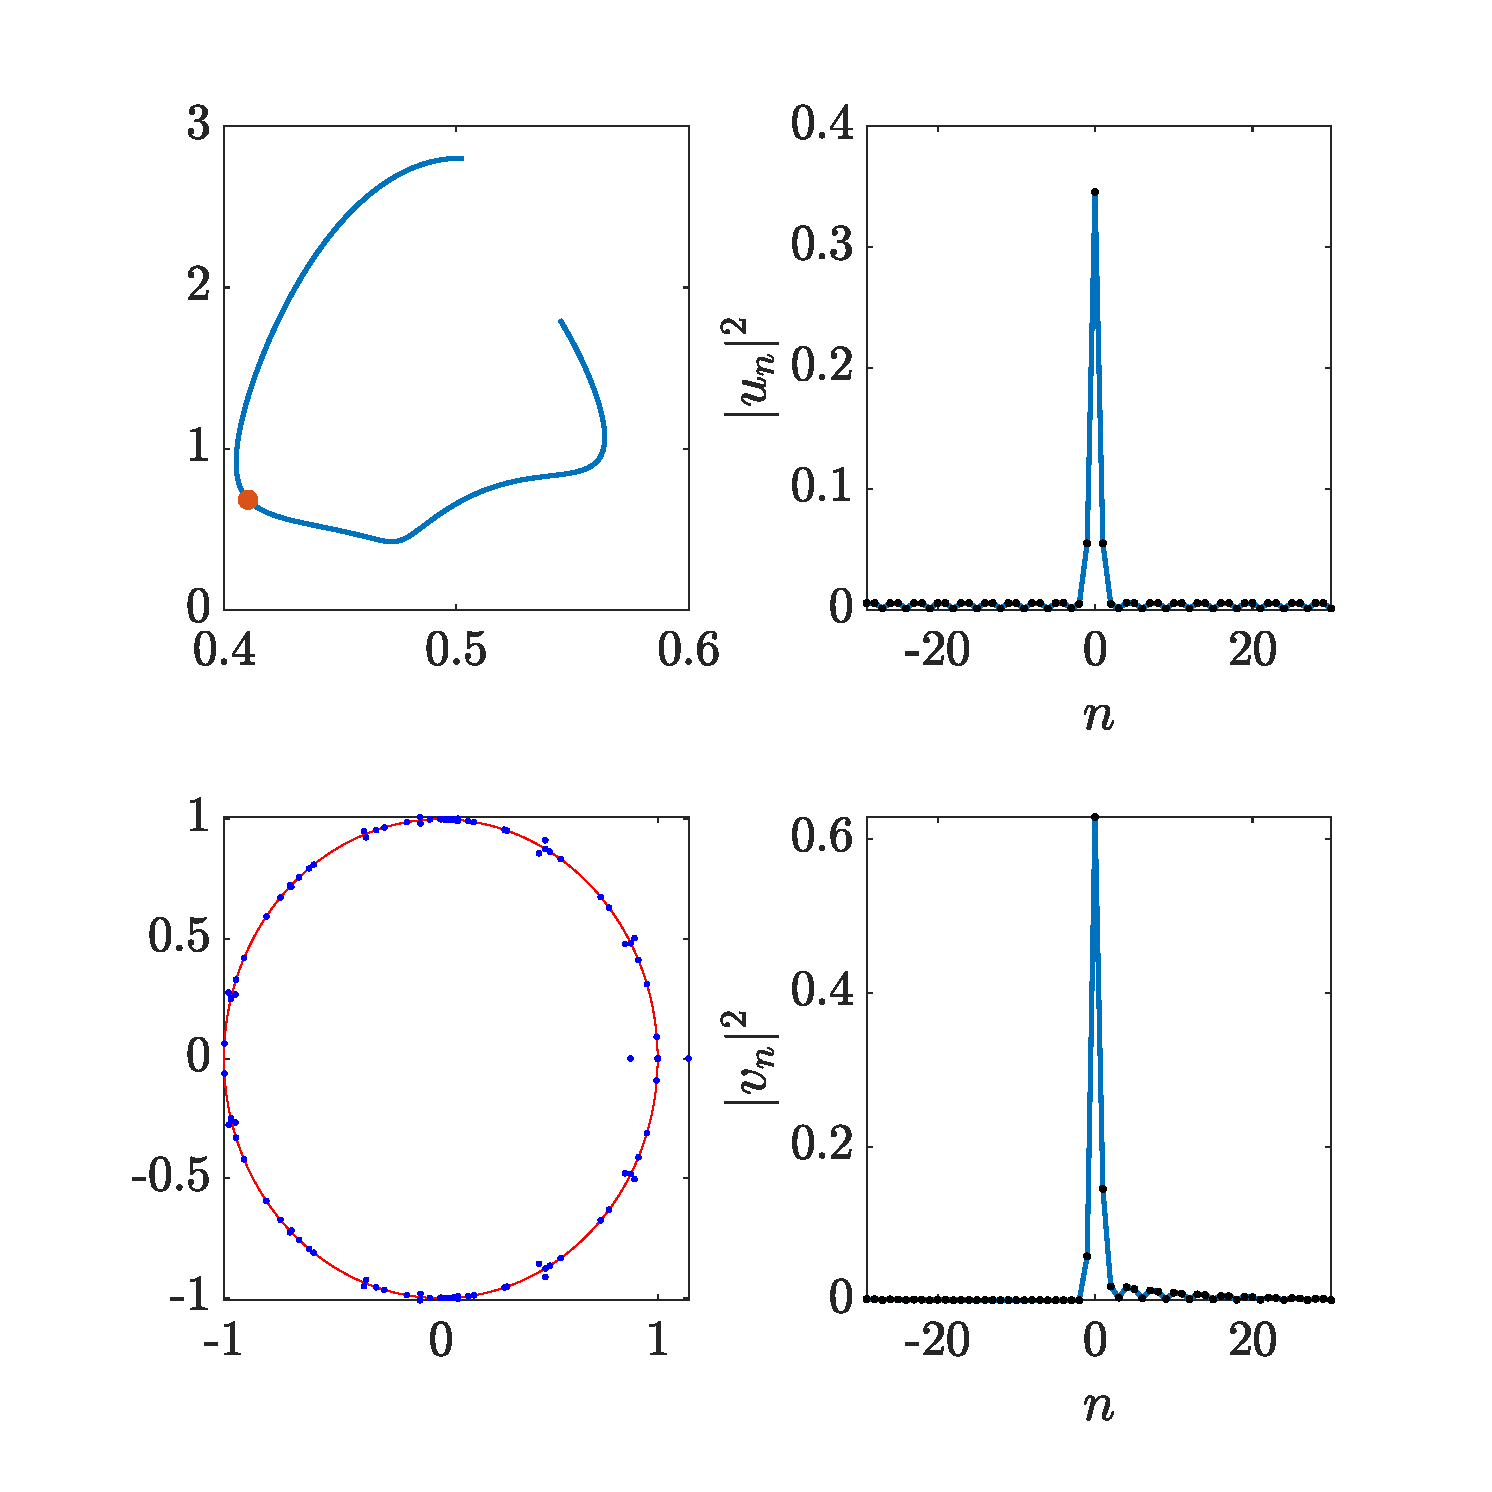
\includegraphics[width=12cm]{leftafterinstabilityL}
    \caption{Solution after the instability on left of bifurcation diagram for $m=60$ (top right). Position on bifurcation diagram shown in top left. Floquet spectrum in bottom left. Corresponding eigenfunction to real eigenvalue is localized (bottom right). $C = 0.4104$}
    \label{fig:leftinstabL}
\end{figure}

\begin{figure}[H]
    \centering
    \begin{tabular}{cc}
    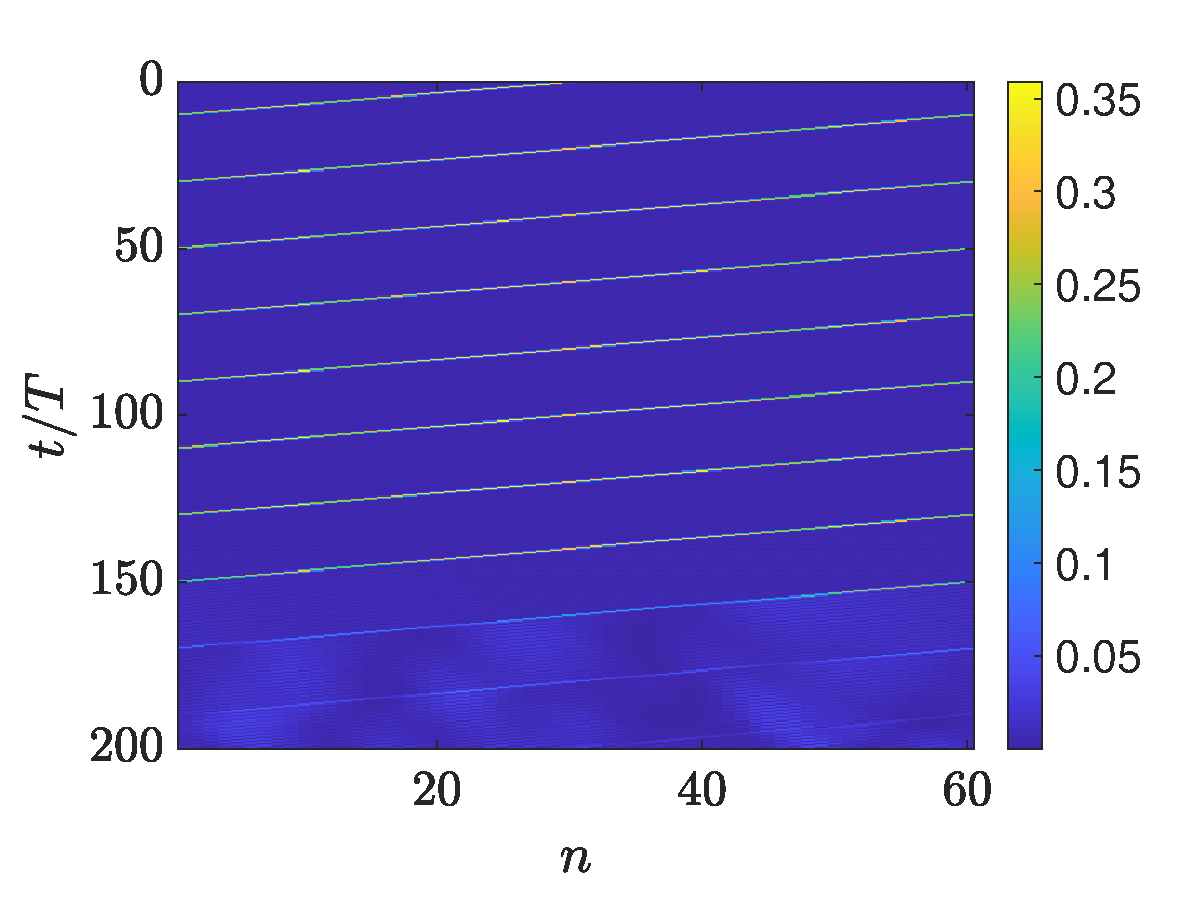
\includegraphics[width=7cm]{leftafterinstabilityLtimestep} &
    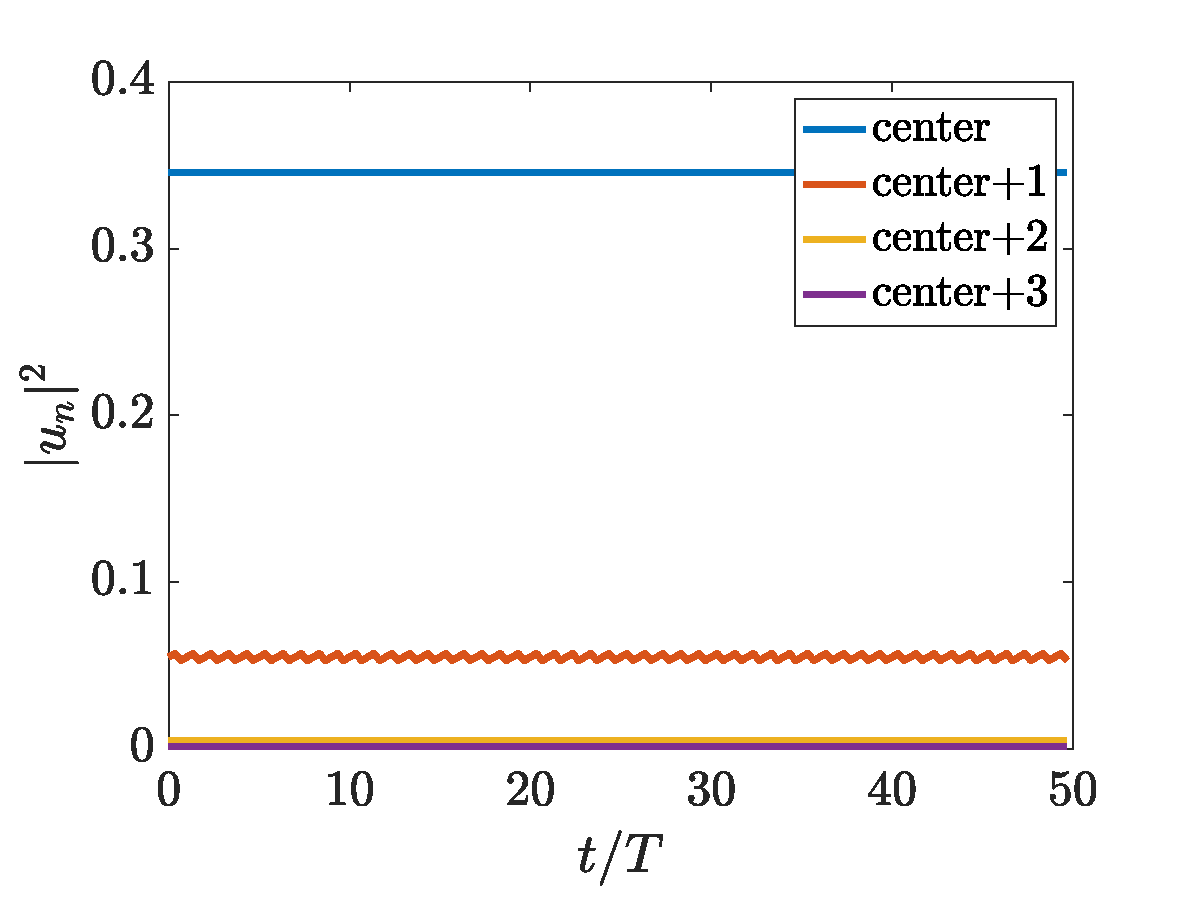
\includegraphics[width=7cm]{leftafterinstabilityLpower} \\ 
    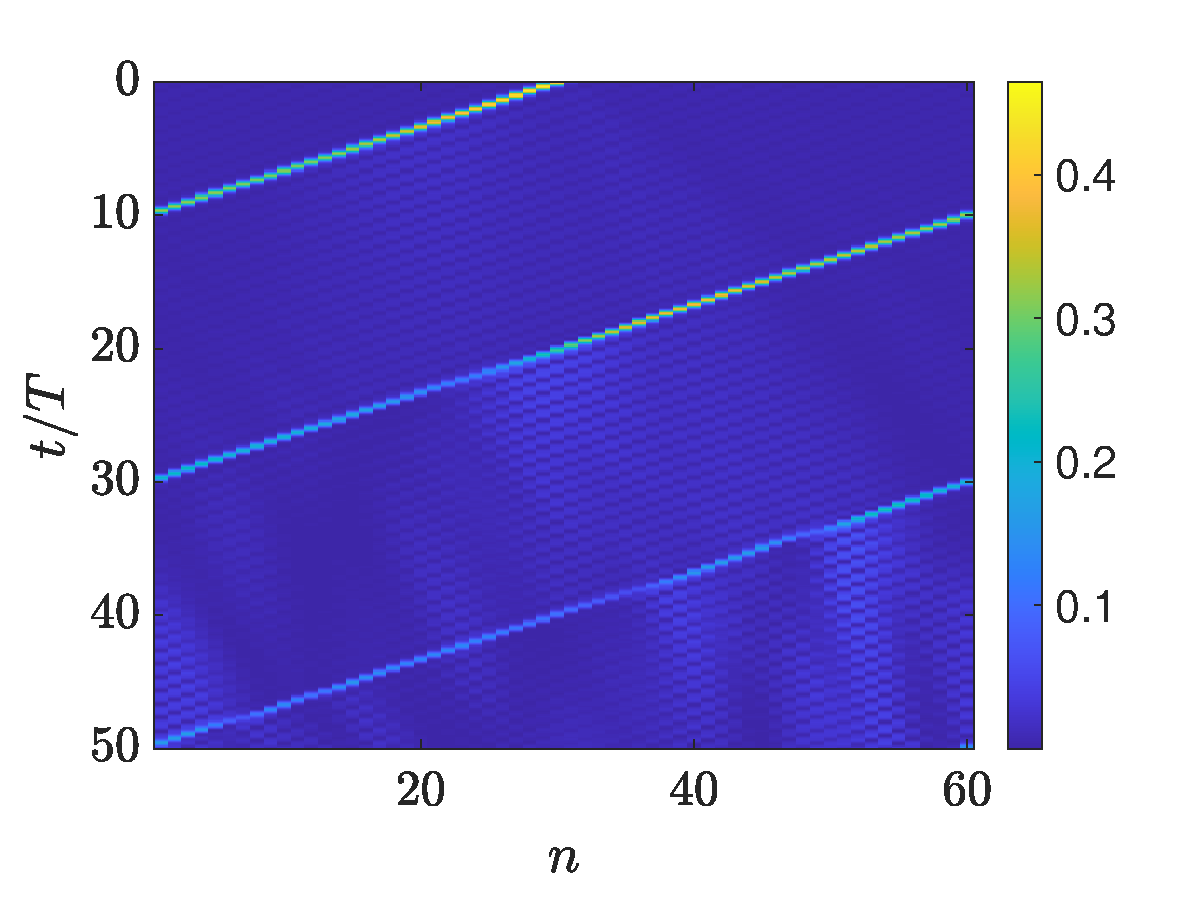
\includegraphics[width=7cm]{leftafterinstabilityLperttimestep} &
    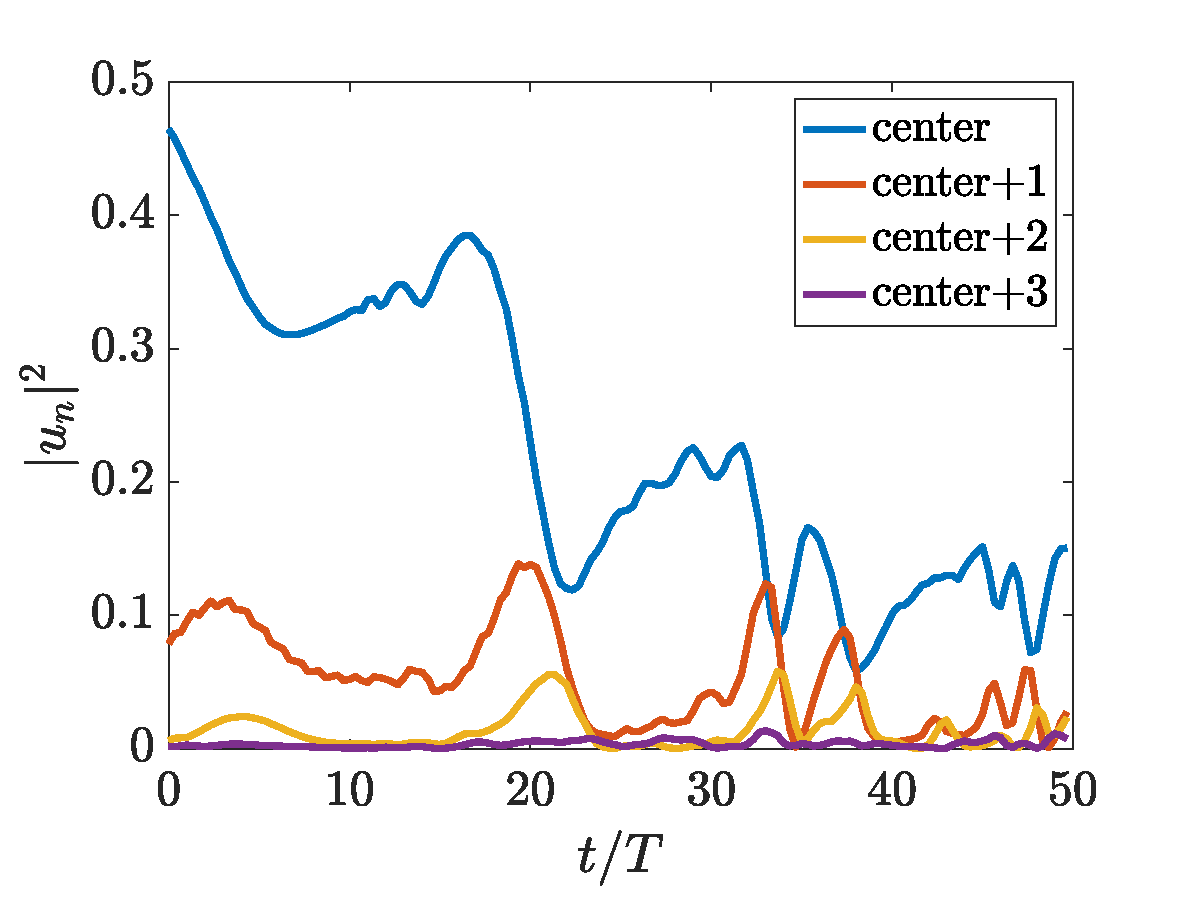
\includegraphics[width=7cm]{leftafterinstabilityLpertpower}
    \end{tabular}
    \caption{Colormap showing time evolution of $|u_n|^2$ (left) and power of center site and right neighbors of left-moving solution for solution after the instability on left of bifurcation diagram for $m=60$. Top is unperturbed solution, bottom is perturbed by adding $\delta$ times the eigenfunction corresponding to the unstable, real Floquet eigenmode. $\delta = 0.4$, $C=0.4104$. }
    \label{fig:leftinstabLpert}
\end{figure}

\section{Right moving solution}

\begin{figure}[H]
    \centering
    \begin{tabular}{ccc}
    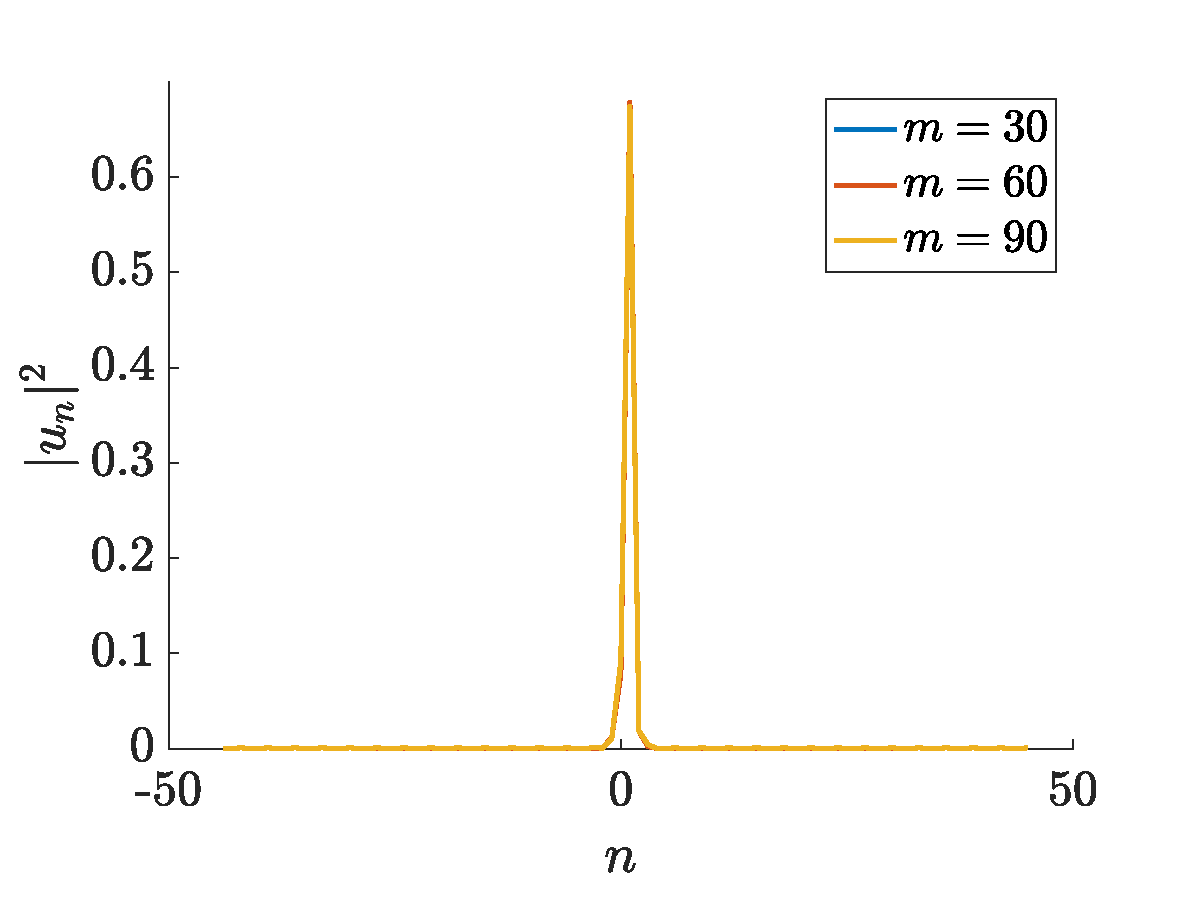
\includegraphics[width=5cm]{rightm} &
    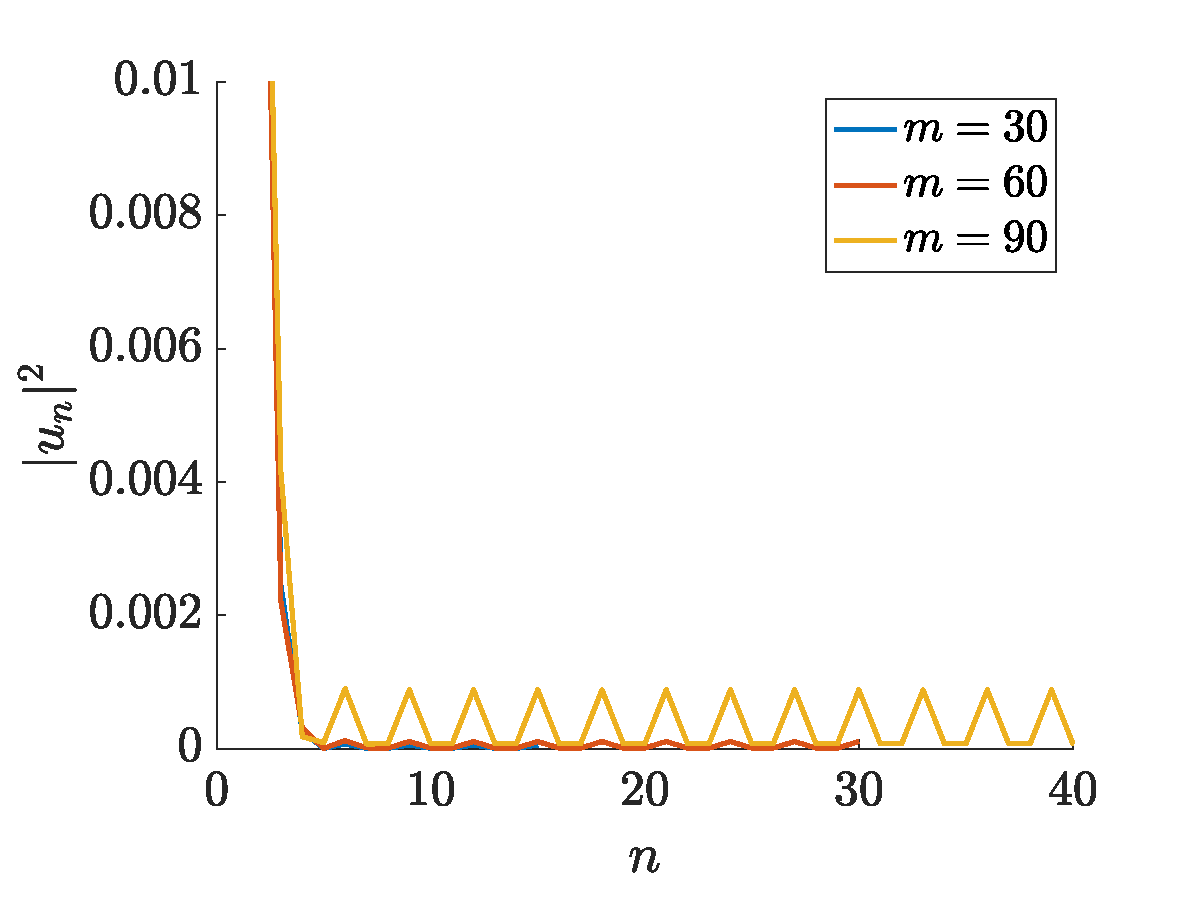
\includegraphics[width=5cm]{rightmnanop} &
    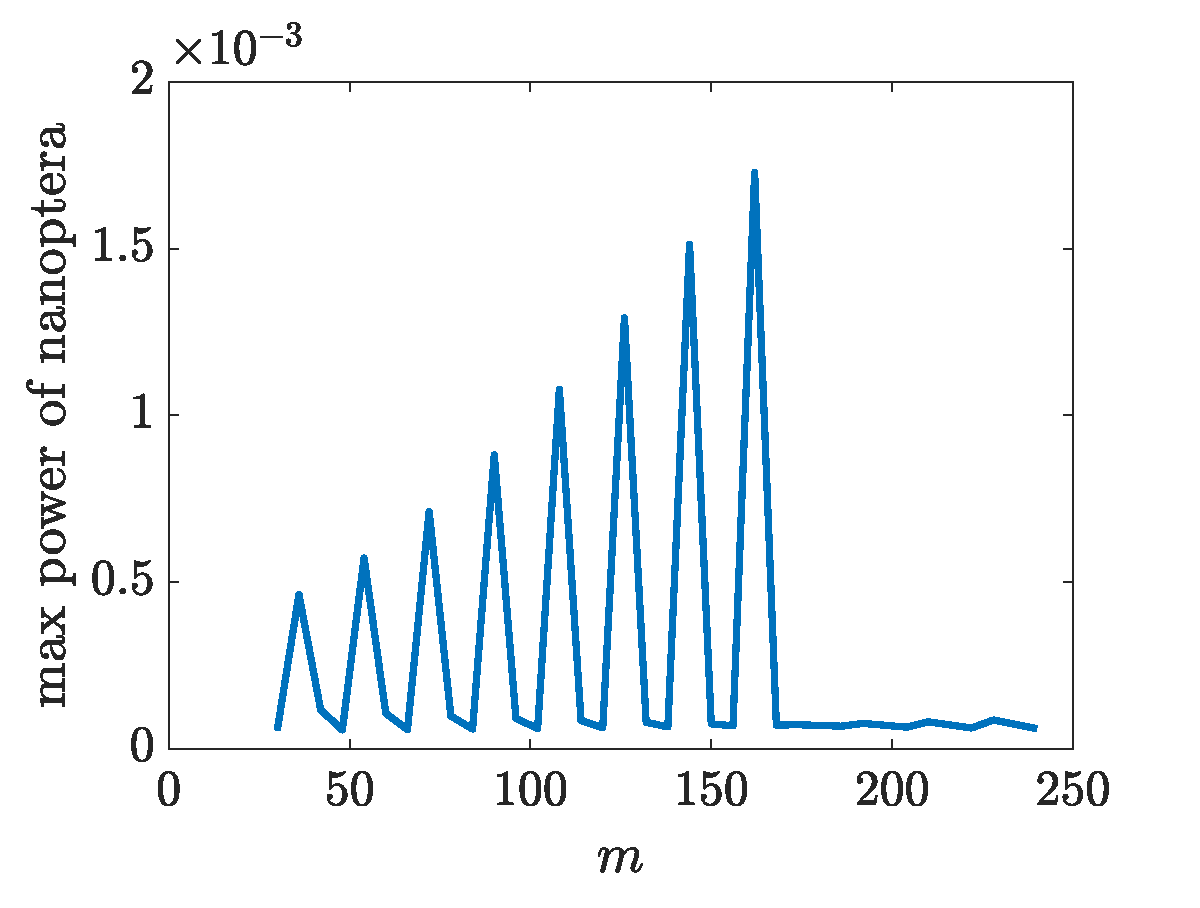
\includegraphics[width=5cm]{rightmnanopmax} \\
    \end{tabular}
    \caption{Right-moving solution for three values of $m$ (left), zoom on nanoptera tails of these solutions (center), max power of nanoptera vs $m$ (right). $J_0 = 0.05$, $C = 0.5$, $g=1$.}
    \label{fig:right1}
\end{figure}

\begin{figure}[H]
    \centering
    \begin{tabular}{ccc}
    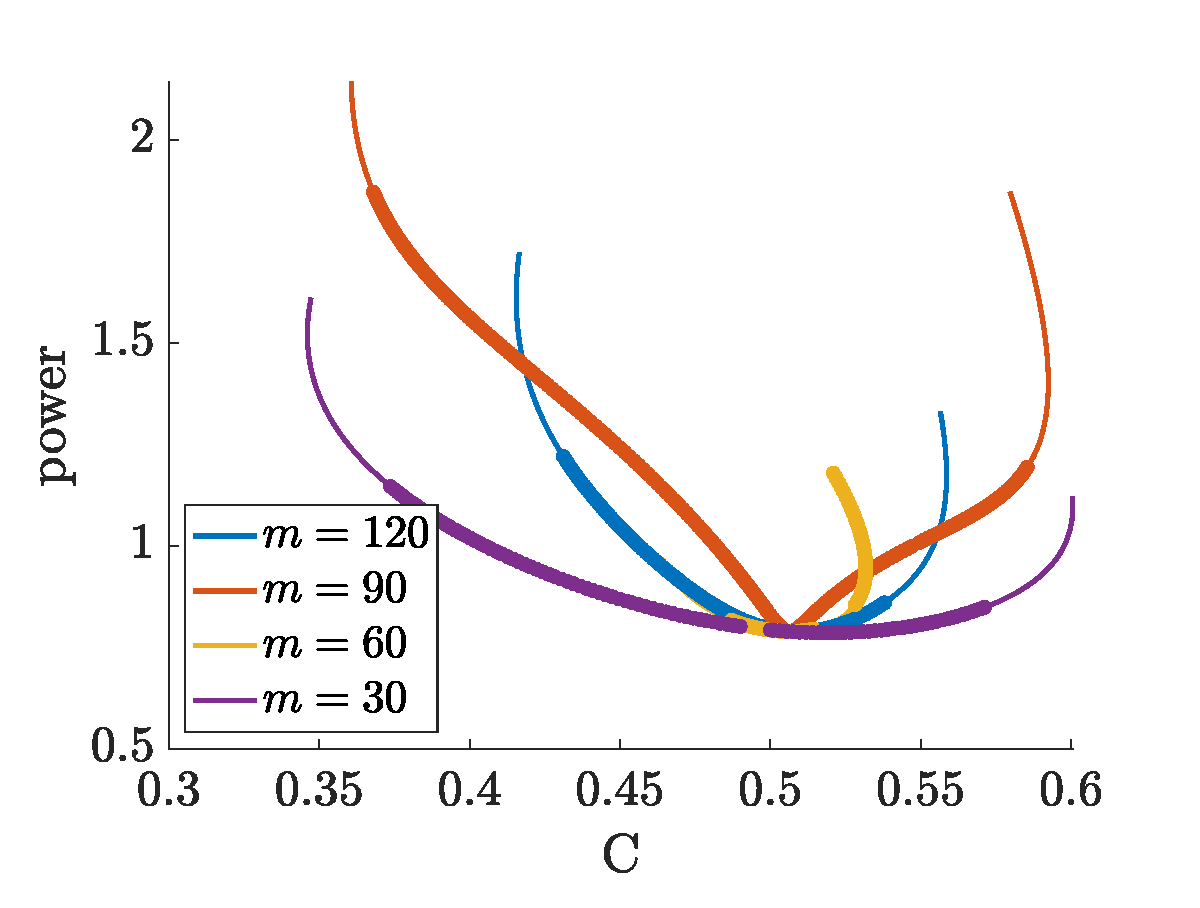
\includegraphics[width=5cm]{rightBD1} &
    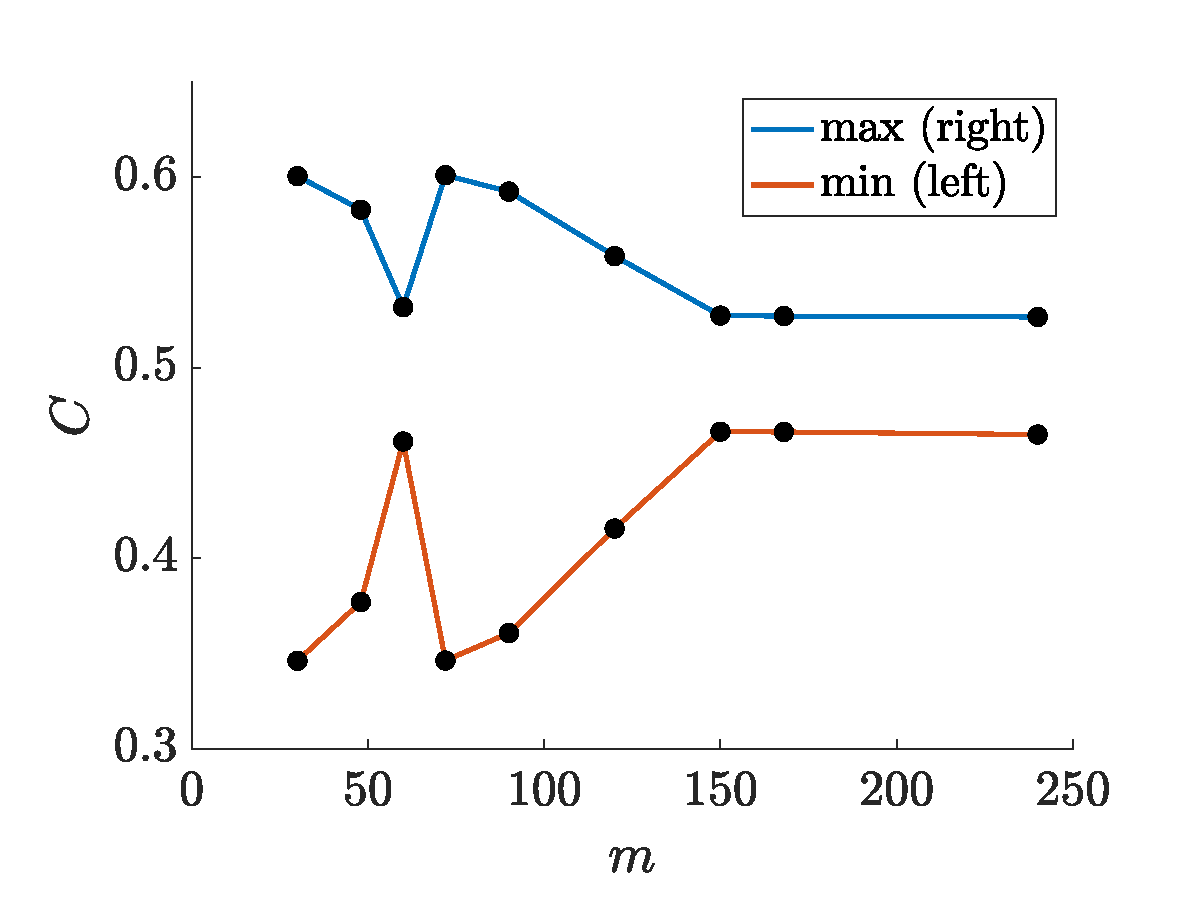
\includegraphics[width=5cm]{rightmaxminC} 
    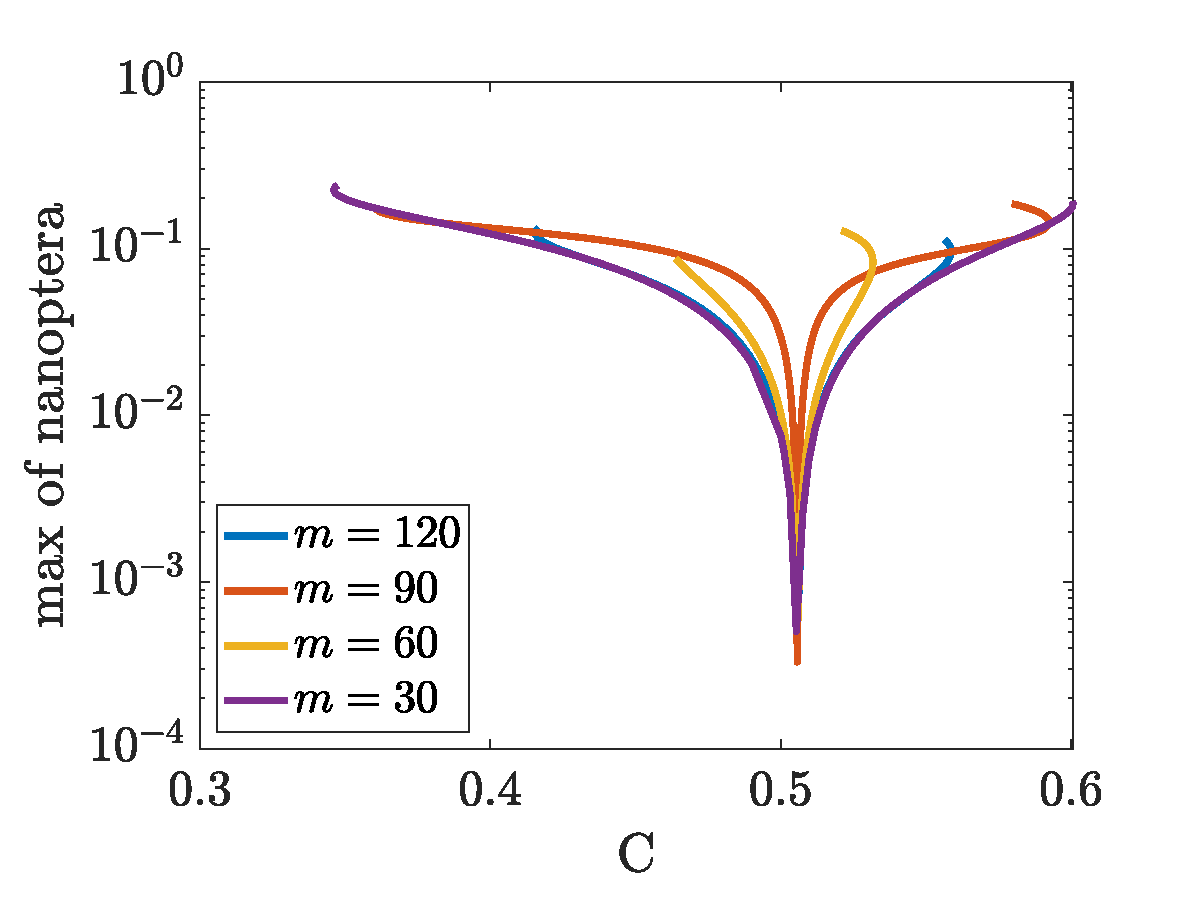
\includegraphics[width=5cm]{rightBDnanop} 
    \end{tabular}
    \caption{Left: Bifurcation diagram for continuation in $C$ for different lattice sizes $m$. Spectrally stable portion is thicker line. Spectral stability here is defined by having no purely real Floquet multipliers greater than 1. Multipliers off of the unit circle resulting from band collisions are not counted (these are essentially always present). For all values of $m$, spectral instability results from a collision of Floquet multipliers on unit circle at $(1,0)$, which leads to a real eigenvalue greater than 1. This occurs for both the right and left instabilities on the bifurcation diagram. See figures below for Floquet spectrum and form of corresponding eigenfunction.
    Center: max and min of $C$ on bifurcation diagram for varying $m$. 
    Right: max of nanoptera vs. $C$.}
    \label{fig:right2}
\end{figure}

\begin{figure}[H]
    \centering
    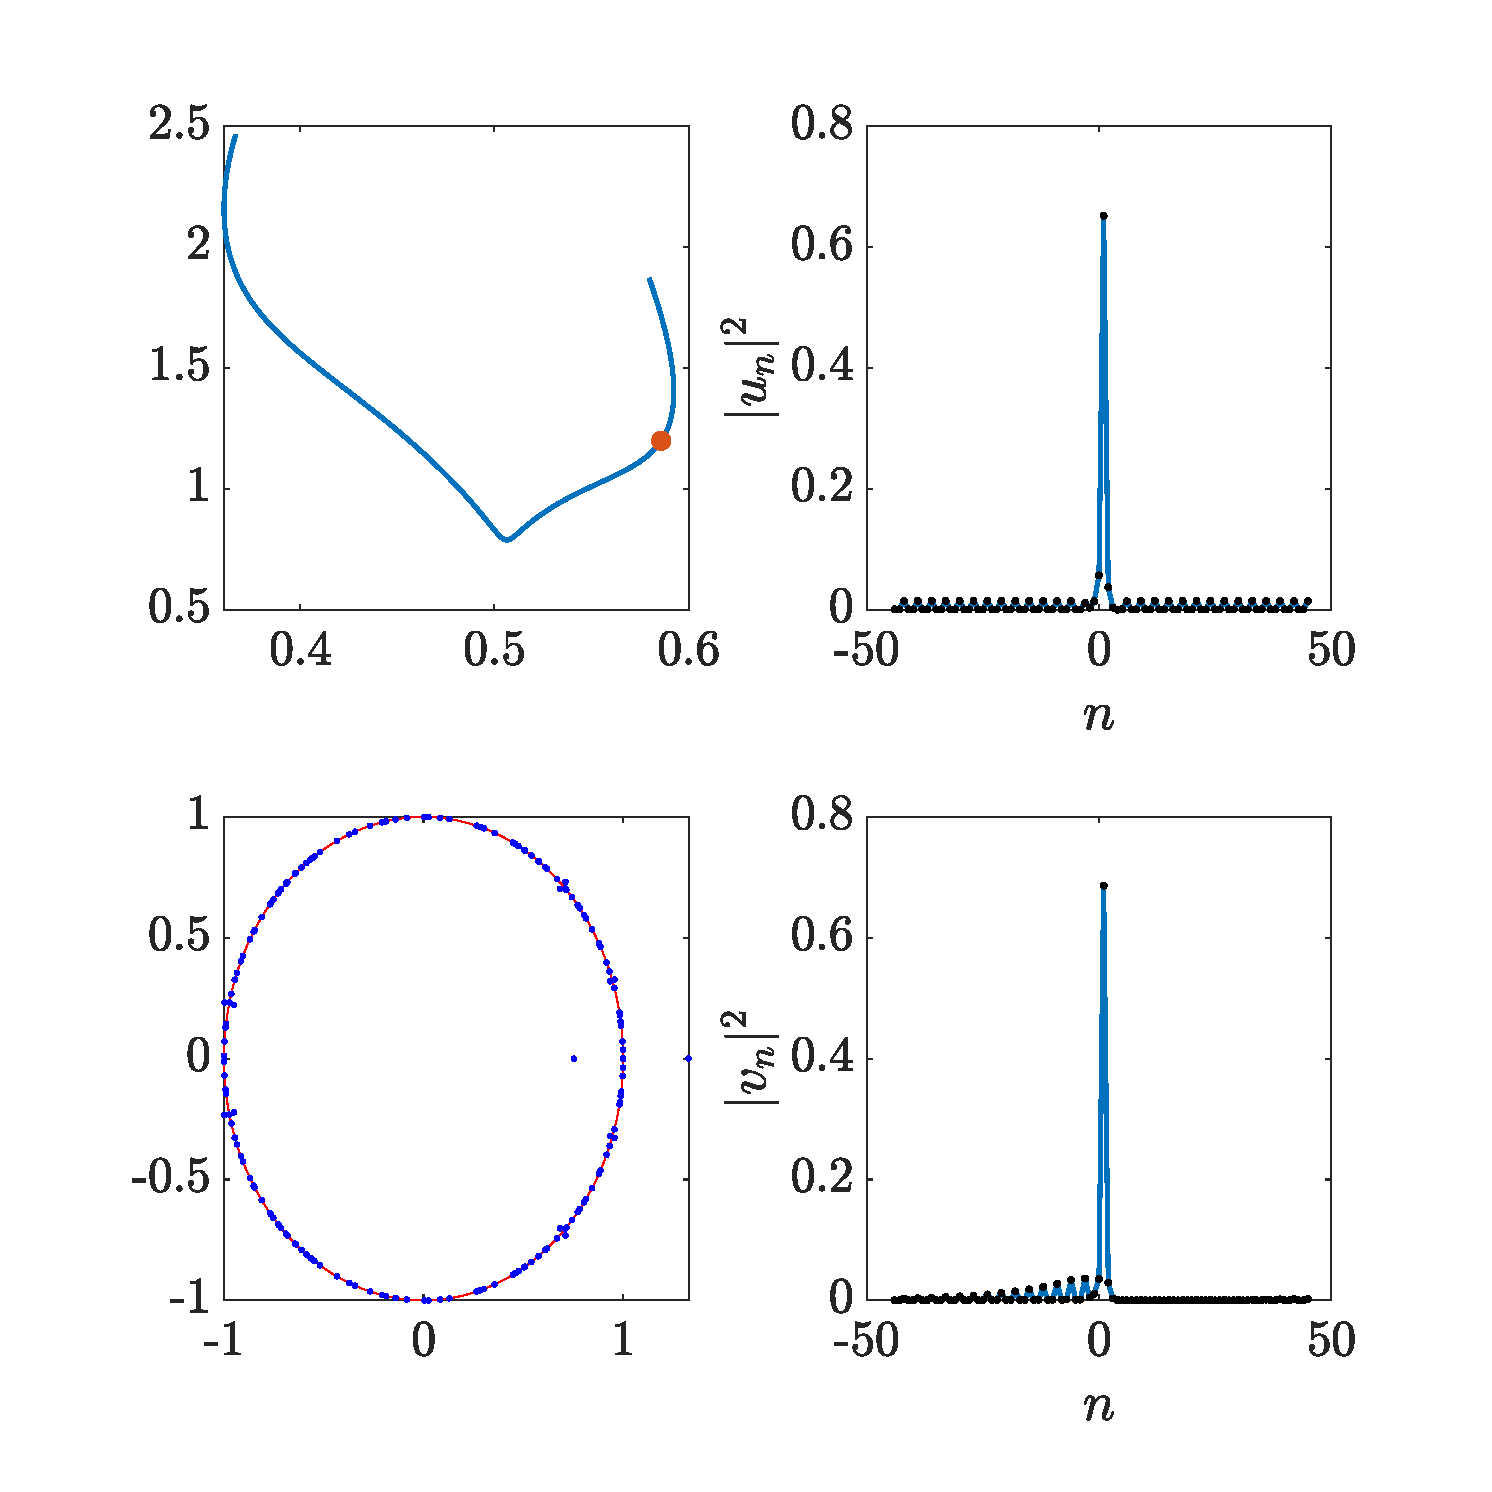
\includegraphics[width=12cm]{rightafterinstabilityR}
    \caption{Solution after the instability on right of bifurcation diagram for $m=90$ (top right). Position on bifurcation diagram shown in top left. Floquet spectrum in bottom left. Corresponding eigenfunction to real eigenvalue is localized (bottom right). $C = 0.5859$}
    \label{fig:rightinstabR}
\end{figure}

\begin{figure}[H]
    \centering
    \begin{tabular}{cc}
    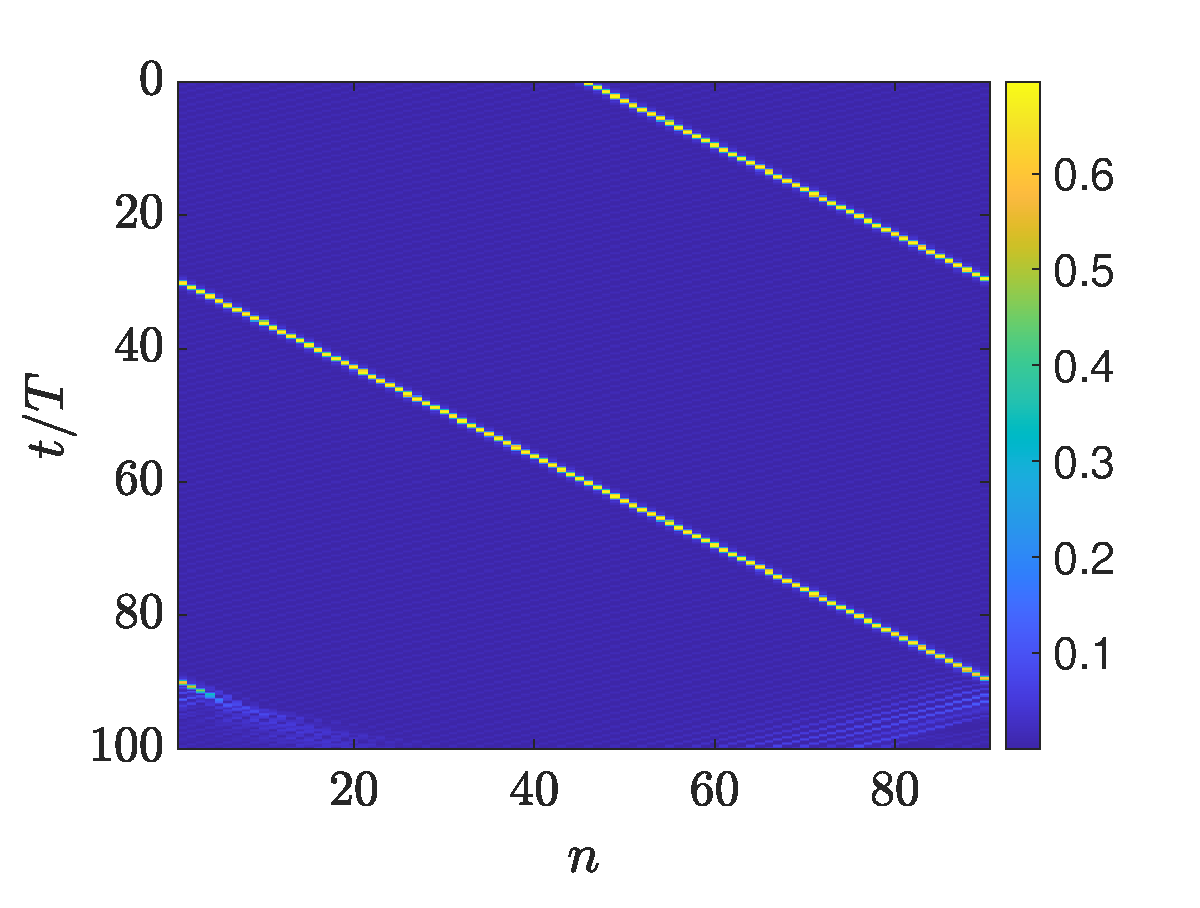
\includegraphics[width=7cm]{rightafterinstabilityRtimestep} &
    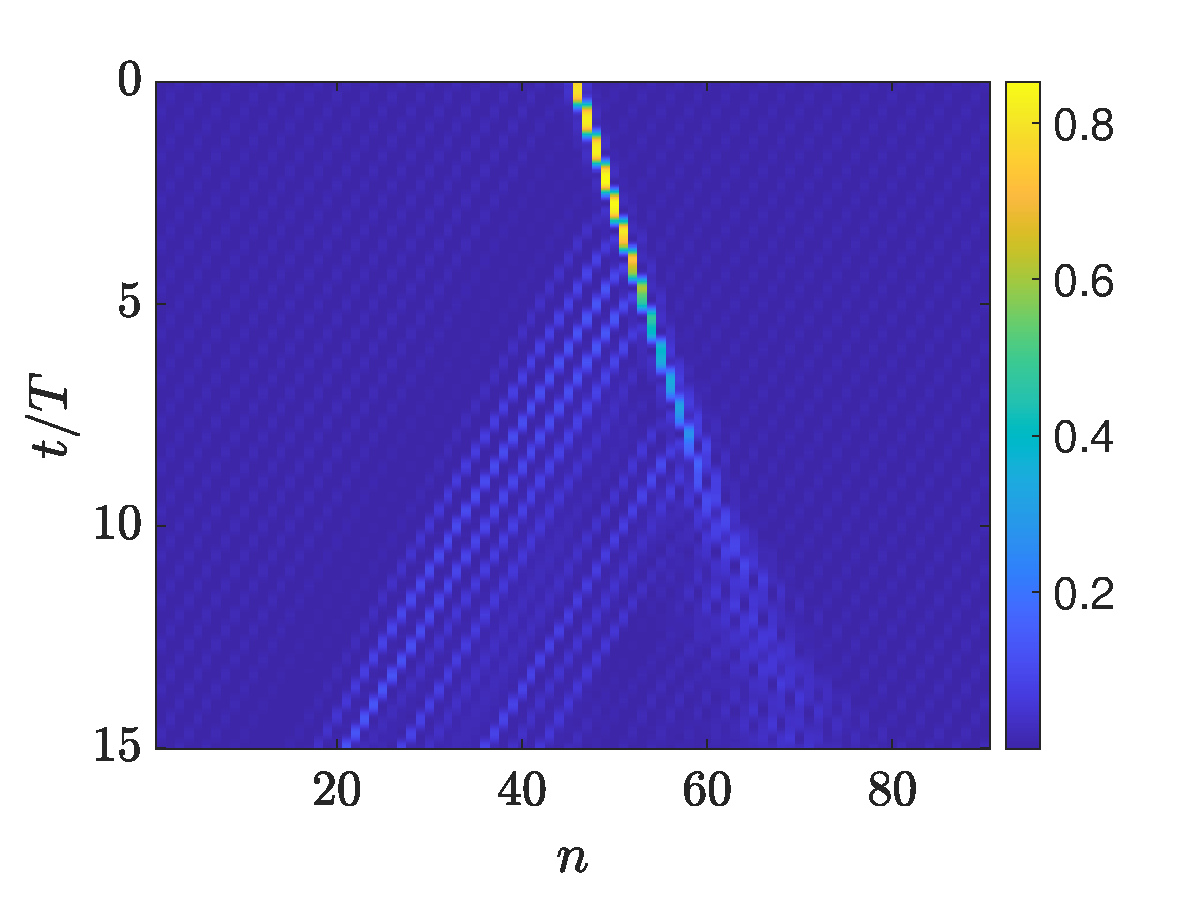
\includegraphics[width=7cm]{rightafterinstabilityRperttimestep}
    \end{tabular}
    \caption{Colormap showing time evolution of $|u_n|^2$ of unperturbed (left) and perturbed (right) right-moving solution for solution after the instability on right of bifurcation diagram for $m=90$. Top is unperturbed solution, bottom is perturbed by adding $\delta$ times the eigenfunction corresponding to the unstable, real Floquet eigenmode. $\delta = 0.4$, $C=0.5859$. }
    \label{fig:rightinstabRpert}
\end{figure}

\begin{figure}[H]
    \centering
    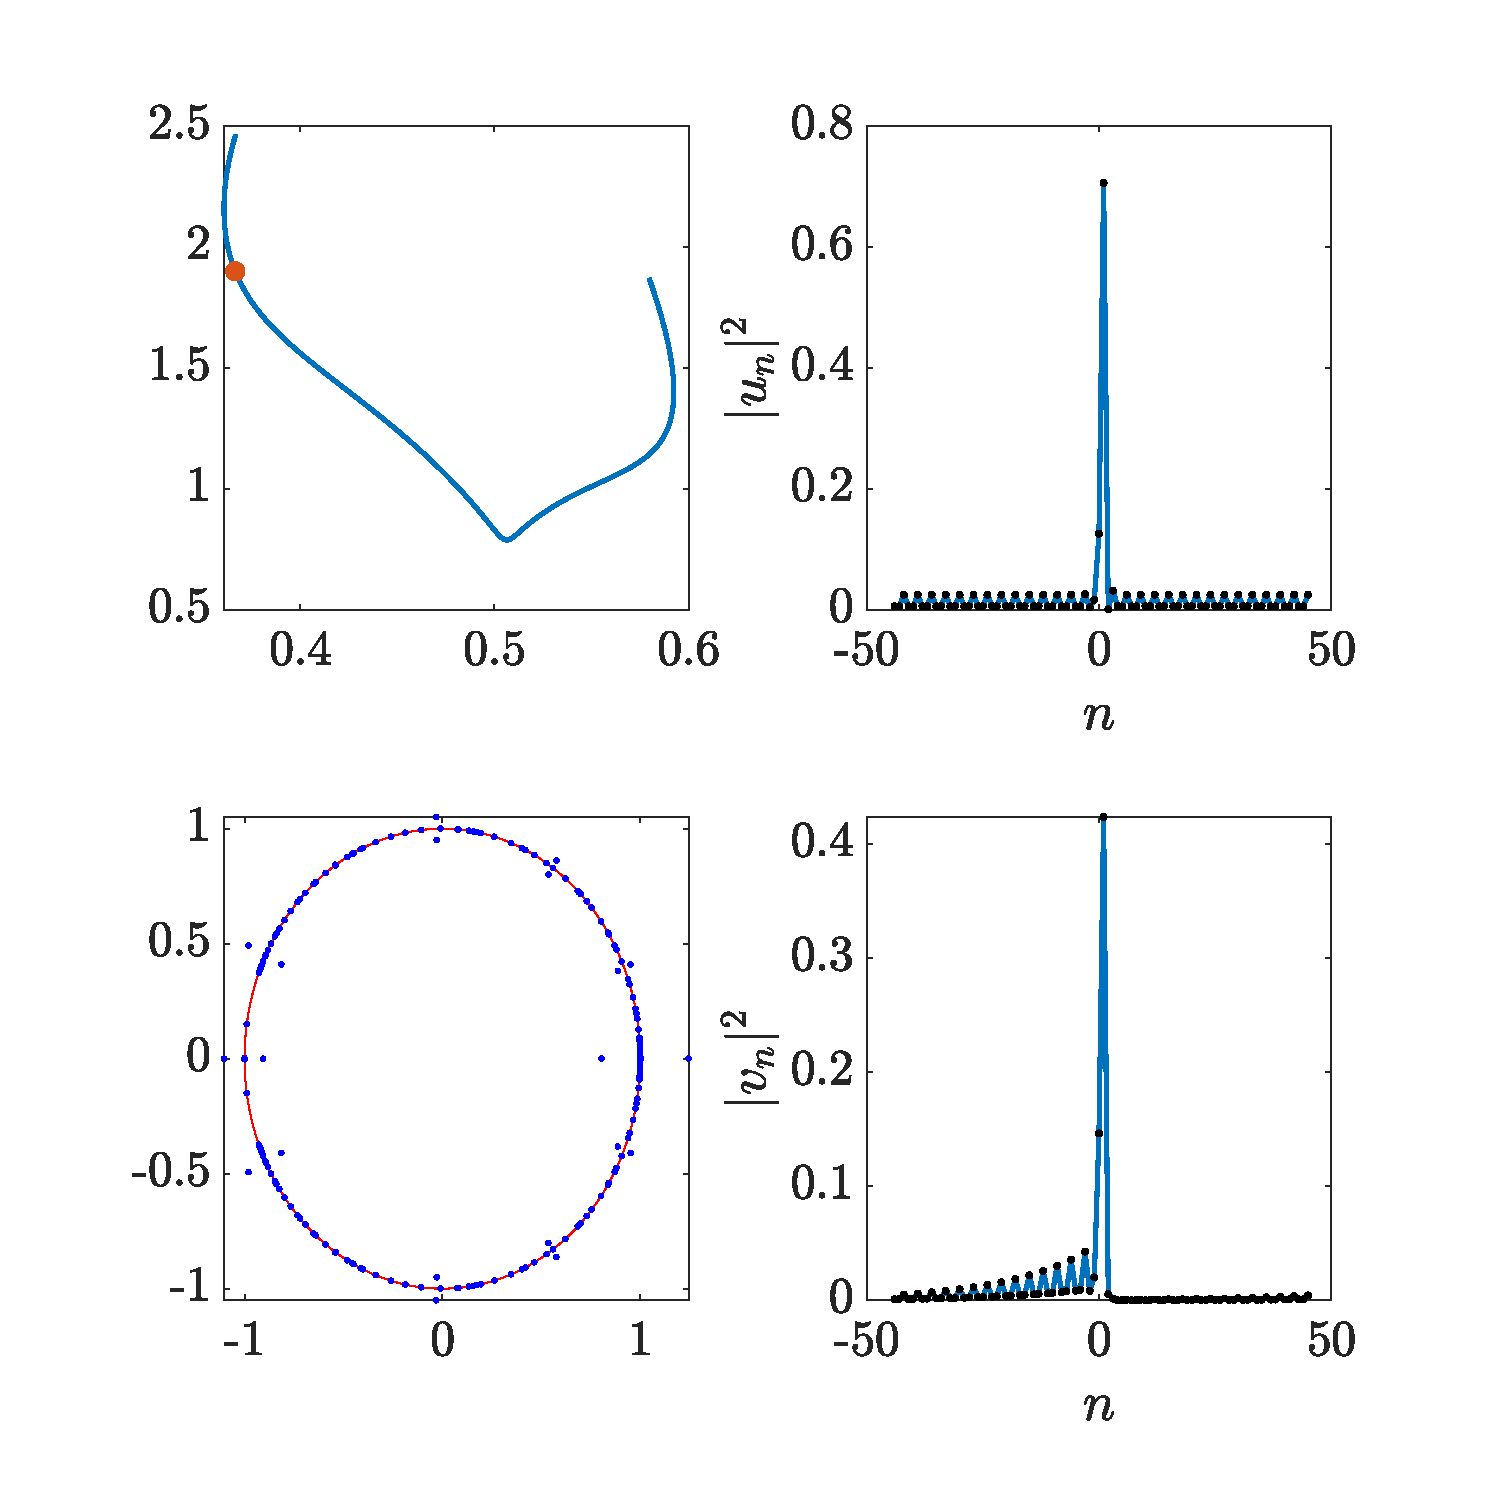
\includegraphics[width=12cm]{rightafterinstabilityL}
    \caption{Solution after the instability on left of bifurcation diagram for $m=90$ (top right). Position on bifurcation diagram shown in top left. Floquet spectrum in bottom left. Corresponding eigenfunction to real eigenvalue is localized (bottom right). $C = 0.3665$}
    \label{fig:rightinstabL}
\end{figure}

\begin{figure}[H]
    \centering
    \begin{tabular}{cc}
    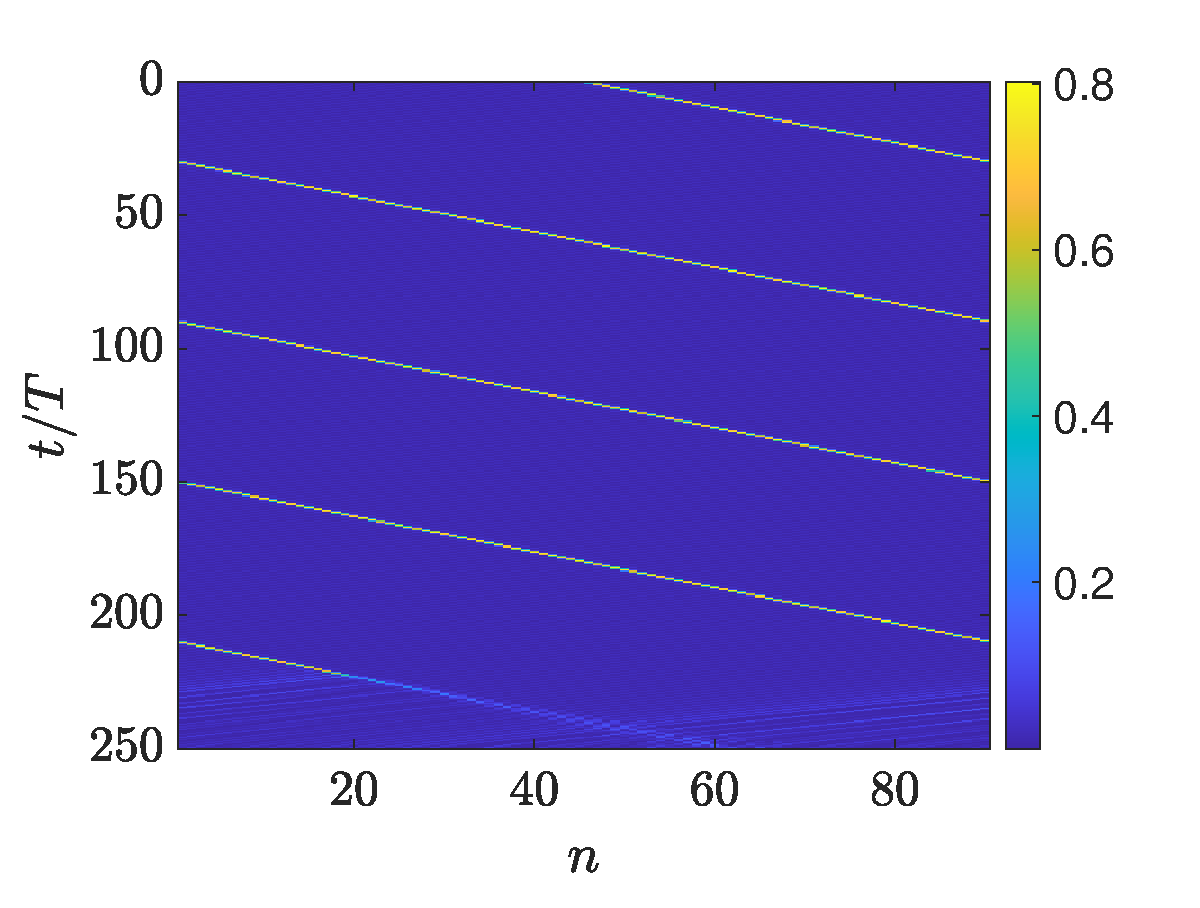
\includegraphics[width=7cm]{rightafterinstabilityLtimestep} &
    \includegraphics[width=7cm]{rightafterinstabilityLperttimestep}
    \end{tabular}
    \caption{Colormap showing time evolution of $|u_n|^2$ of unperturbed (left) and perturbed (right) right-moving solution for solution after the instability on left of bifurcation diagram for $m=90$. Top is unperturbed solution, bottom is perturbed by adding $\delta$ times the eigenfunction corresponding to the unstable, real Floquet eigenmode. $\delta = 0.4$, $C = 0.3665$. }
    \label{fig:rightinstabLpert}
\end{figure}


\bibliographystyle{amsplain}
\bibliography{main.bib}

\end{document}